\chapter{Разработка схем для многократного вовлечения регенерированного урана в топливный цикл}\label{ch:ch3}

Рассмотренные в предыдущих главах каскадные схемы, частично или полностью позволяют решить проблемы, связанные с присутствием в урановой смеси изотопов $^{232,233,234}$U. Однако при использовании таких схем для возврата состава загрязненного регенерированного урана, прошедшего несколько циклов использования в качестве топлива легководных реакторов, расход регенерированного урана на единицу продукта, как правило, таков, что не позволяет полностью замкнуть цикл по урану -- добиться равенства масс регенерата, полученного из 1 кг ОЯТ и затраченного на производство 1 кг регенерированного топлива.

Отсюда вытекает потребность в разработке каскадных схем, которые смогут не только обеспечить выполнение требований по содержанию четных изотопов в продукте, но и израсходовать на производство низкообогащенного урана 100\% имеющегося в распоряжении регенерированного урана. Второе условие позволяет вернуть в топливный цикл весь выделенный из ОЯТ регенерат вне зависимости от его изотопного состава, что гарантирует возможность использования подобной схемы для обогащения неоднократно облученного регенерата урана.

\section{Схема двойного каскада с НОУ-разбавителем}
\subsection{Описание схемы}

Развитием идеи двойного каскада является модификация в виде дополнительного использования в качестве разбавителя низкообогащенного урана, полученного из природного урана. Такая схема, представленая на рис. \ref{p2left} была впервые предложена в работе \cite{vodolazskihSposobIzotopnogoVosstanovleniya2006}. Принцип работы такой схемы опирается на идею <<пространственного>> разделения на легкую ($^{232,233,234}$U) и тяжелую фракции ($^{235,238}$U), предложенную в двойном каскаде, и заключается в следующем. 

\begin{figure}[ht]
    \centerfloat{
\includegraphics[scale=0.9]{cascades/p2left}}
    \caption{Схема модифицированного двойного каскада для обогащения регенерированного урана. Обозначения: $E$ -- поток регенерированного урана; $P_1$ -- поток отбора первого каскада, выступающий питанием второго каскада; $P_2$ -- поток отбора второго каскада; $W_1$ -- поток отвала первого каскада; $W_2$ -- поток тяжелой фракции (условный «отвал») второго каскада; $P_0$ -- поток НОУ-разбавителя; $P$ -- финальный продукт (товарный низкообогащенный уран (НОУ))}\label{p2left}
\end{figure}

В первом каскаде исходный материал обогащается по изотопам $^{232,233,234,235,236}$U, а во втором каскаде смесь делится на две фракции, так, чтобы в тяжелой фракции преимущественно сконцентрировался продукт с пониженным содержанием $^{232,233,234}$U по отношению к питающей второй каскад смеси. Таким образом, в первом каскаде, на одном из концов, смесь обогащают по легким изотопам (в первую очередь $^{232,233,234,235}$U) в потоке $P_1$.
В $P_1$ концентрация $^{235}$U выбирается в диапазоне от 5\% до 20\%, поскольку ее величина должна быть больше требуемой в конечном продукте, ввиду того, что во втором каскаде получаемый продукт будет обеднен по $^{235}$U. Далее, полученный в первом каскаде обогащенный уран направляется на вход второго каскада, где он разделяется на 2 группы: в первой концентрируются легкие изотопы и $^{235}$U, во второй легкие изотопы обедняются, параллельно с относительно небольшим снижением концентрации $^{235}$U (на 0.5–2.5\%). В этом случае число ступеней в части каскада, заключенной между потоками $P_1$ и потоком тяжелой фракции второго каскада, будет в несколько раз меньше, чем в части между потоками $P_1$ и $P_2$. При таких условиях поток тяжелой фракции второго каскада будет близок по величине к потоку питания второго каскада.
Выбор концентрации $^{235}$U в потоке отбора второго каскада зависит от наличия ограничения на производство высокообогащенного урана \cite{brownOriginsSignificanceLimit2016}.

Финальным шагом к получению конечного НОУ-продукта является разбавление потока тяжелой фракции второго каскада $W_2$ сырьем, не содержащим искусственных изотопов урана для выполнения ограничений по $^{232}$U и $^{236}$U. В этом шаге и заключается отличие этой схемы от схемы двойного каскада. При этом для выполнения условия полного возврата регенерата в цикл пропорция смешивания фактически является заранее заданной, поскольку к этому моменту известна пропорция потоков второго каскада, и также известен расход регенерата на единицу конечного продукта. Единственным параметром, позволяющим влиять на концентрацию $^{235}$U в товарном продукте является концентрация данного изотопа в разбавителе (поток $P_0$ на схеме).
% Подмешивание НОУ-разбавителя позволяет добиться требуемых пропорций вовлечения облученного топлива в воспроизводство свежего НОУ-топлива или, иными словами, выполнения условия полного использования регенерата. Для строгого соблюдения такой заранее определенной пропорции, вычисляется и пропорция подмешиваемого НОУ-разбавителя, легко рассчитываемая на основании параметров двойного каскада. Для этого, из известных соотношений в двойном каскаде $\frac{W_{2}}{P_{1}}$ и $\frac{P_{1}}{RepU}$, а также желаемого соотношения $\frac{RepU}{P}$, вычисляется пропорция $W_2$ к конечному продукту $\frac{W_{2}}{P}$, откуда, вычитая ее из единицы, можно получить соотношение дополнительного НОУ-разбавителя к финальному НОУ-продукту $\frac{P_{0}}{P}$, где $RepU$ -- это поток регенерата, а $P$ -- поток финального НОУ-продукта.

Поскольку питанием первого каскада выступает только регенерат, а питанием второго -- полученный из него средне-обогащенный регенерат, то поток тяжелой фракции на выходе из второго каскада будет в несколько раз меньше, чем исходный поток регенерата. Иными словами, при такой работе каскад будет обеспечивать перерасход регенерата на единицу продукта. Следовательно, поток разбавителя ($P_{0}$) должен в несколько раз превосходить по величине поток получаемый в тяжелой фракции второго каскада. Однако, если в качестве разбавителя использовать, например, природный уран, это условие может привести к снижению концентрации $^{235}$U ниже требуемой величины. В этой связи целесообразно, в качестве разбавителя использовать низкообогащенный уран, поскольку ввиду более высокой концентрации $^{235}$U по отношению к природной смеси можно увеличить пропорцию разбавителя и разбавляемого вещества. Однако, в качестве сырья $F_0$ для наработки разбавителя, наряду с природным ураном, может быть использован и складской обедненный уран, нарабатывавшийся в ходе производства обогащенного урана из природного урана.
% Выбор ОГФУ в качестве сырья НОУ-разбавителя позволяет не расходовать природный уран в процессе рециклирования топлива, ценой дополнительных затрат разделительной работы, что может оказаться привлекательной возможностью в некоторых случаях, особенно при росте цены на природный уран.

Таким образом, первые два каскада в данной схеме работают только с регенерированным ураном, позволяя частично отделить $^{235}$U от более легких $^{232}$U и $^{234}$U. Роль третьего каскада состоит в наработке разбавителя $P_{0}$, необходимого для формирования требуемой массы конечного продукта с одновременным выполнением условий по четным изотопам в этом продукте.

% Предварительная оценка параметров каскадной схемы необходимых для получения НОУ-продукта требуемых качеств, показывает, что величина потока разбавителя $P_0$ должна в несколько раз превосходить по величине поток тяжелой фракции второго каскада $W_2$. Если бы в качестве разбавителя использовали природный уран, это бы привело к снижению концентрации $^{235}$U в результирующей смеси ниже требуемой величины. Именно поэтому в схеме предусмотрен дополнительный каскад, нарабатывающий низкообогащенный уран в потоке $P_0$ из смесей природного (нереакторного) происхождения -- природного или обедненного урана.

\subsection{Пример применения схемы двойного каскада с НОУ-разбавителем} 

Рассмотрим пример, позволяющий проиллюстрировать принцип действия подобной схемы каскада для обогащения регенерированного урана, испытавшего несколько циклов облучения (таблица \ref*{is_compositions_2_5}) \cite{smirnovObogashchenieRegenerirovannogoUrana2018}. Расчеты проведены при следующих условиях: обогащение по изотопу  $^{235}$U составляло 4.95\%; относительный коэффициент разделения компонентов $^{235}$UF$_{6}$ и $^{238}$UF$_{6}$ принят равным 1.2 \cite{smirnovKaskadnyeShemyZadachah2012}; предельно допустимая концентрация изотопа $^{232}$U в НОУ не должна превышать величину $5\cdot10^{-7}$\% \cite{blandinskiySoglasovannyyPodhodModelirovaniyu2018}; потерю реактивности из-за присутствия $^{236}$U компенсировали добавочным обогащением по $^{235}$U. Заданный расход регенерированного урана на единицу продукта: 930 г на 1 кг, что примерно соответствует условиям выгорания топлива в реакторе ВВЭР-1000 \cite{smirnovEvolutionIsotopicComposition2012}. В качестве расчетной модели в настоящей работе использована модель <<квазиидеального>> каскада \cite{sazykinKvaziidealnyeKaskadyDlya2000} с несмешиванием по относительным концентрациям выбранной пары компонентов (R-каскада) \cite{delagarzaMulticomponentIsotopeSeparation1961}. Данная модель широко используется при моделировании процессов разделения многокомпонентных изотопных смесей, в первую очередь, для изучения физических закономерностей процессов массопереноса в разделительных каскадах, а также для оценки их ключевых параметров (числа ступеней, номера ступени подачи питания, минимального числа разделительных элементов, затрат работы разделения и др.). При этом показано, что R-каскады характеризуются параметрами, близкими к параметрам каскадов, оптимизированных по величине суммарного потока. Последнее обстоятельство фактически означает минимальность затрат работы разделения в случае обогащения регенерированного урана \cite{sulaberidzeSravnenieOptimalnyhModelnyh2008,songComparativeStudyModel2010}. Такие понятия как <<работа разделения>> и <<единица работы разделения (ЕРР)>> принципиально введены для двухкомпонентных смесей. Для многокомпонентной смеси и, в том числе, смеси регенерированного урана, понятие работы разделения является условным. Поэтому в приведенных ниже результатах под работой разделения подразумевали условную величину прямо пропорциональную числу газовых центрифуг в каскаде.

Ниже представлены результаты расчета изотопных составов и удельных расходов природного урана и регенерированного урана, а также затрат работы разделения на 1 кг получаемого продукта. На основе серии расчетов для первого R-каскада выбрали условие несмешивания по относительной концентрации компонентов $^{235}$UF$_{6}$ /$^{236}$UF$_{6}$ и величину обогащения по $^{235}$U на уровне 10\%. Получившиеся параметры каскада представлены в таблице \ref{MDKcas1params}. Полученный промежуточный продукт (P1) поступает на вход второго каскада. При этом концентрации $^{235}$U в выходных потоках второго R-каскада с несмешиванием по компонентам $^{234}$UF$_{6}$/$^{235}$UF$_{6}$  приняты равными 20 и 8\%, в обогащенной и обеднееной фракциях, соответственно. Выбор подобных концентраций осуществлен на основе серии предварительных расчетов, целью которых было определить оптимальные значения данных концентраций с точки зрения минимизации расхода природного урана и затрат работы разделения. Рассчитанные параметры второго R-каскада приведены в таблице \ref{MDKcas2params}. Из данных таблиц \ref{MDKcas1params},\ref{MDKcas2params} видно, что расход регенерированного урана в пересчете на единицу потока тяжелой фракции второго каскада ($W_{2}$) заметно превышает требуемую величину 0.93 и составляет $\frac{E}{W_{2}}=\frac{E}{P_{1}} \frac{P_{1}}{W_{2}}=11.104$. Для снижения данной величины полученный регенерат необходимо разбавить. Требуемые отношения потоков, образующих конечный НОУ-продукт, легко рассчитать, а для получения требуемой концентрации $^{235}$U в товарном продукте необходимо подобрать концентрацию разбавителя, опираясь на балансные соотношения.


\begin{table}
\begin{tabular}{|c|c|c|c|c|c|}
    \hline Массовое число & $C_{i}^{P_{1}}, \%$ & $C_{i}^{W_{1}}, \%$ & $C_{i}^{E}, \%$ & $\frac{E}{P_{1}}$ & Удельная работа разделения, отн.ед. \\
    \hline 232 & $9.97 \mathrm{E}-06$ & $1.06 \mathrm{E}-11$ & $1.03 \mathrm{E}-06$ & & \\
    233 & $1.27 \mathrm{E}-05$ & $3.44 \mathrm{E}-10$ & $1.30 \mathrm{E}-06$ & & \\
    234 & $3.78 \mathrm{E}-01$ & $2.37 \mathrm{E}-04$ & $3.91 \mathrm{E}-02$ & & \\
    235 & $9.50 \mathrm{E}+00$ & $1.00 \mathrm{E}-01$ & $1.07 \mathrm{E}-00$ & $9.72$ & 25.6 \\
    236 & $7.89 \mathrm{E}+00$ & $7.06 \mathrm{E}-01$ & $1.45 \mathrm{E}-00$ & & \\
    238 & Остальное & Остальное & Остальное & & \\
    \hline
\end{tabular}
\caption{Параметры первого каскада в схеме}\label{MDKcas1params}
\end{table}

\begin{table}
\begin{tabular}{|c|c|c|c|c|c|c|}
    \hline Массовое & $C_{i}^{P_{2}}, \%$ & $C_{i}^{W_{2}}, \%$ & $C_{i}^{P_{1}}, \%$ & $C_{i}^{P_{0}}, \%$ & $\frac{E}{W_{2}}$ & Удельная работа разделения, отн.ед. \\
    \hline 232 & $3.95 \mathrm{E}-05$ & $5.75 \mathrm{E}-06$ & $9.97 \mathrm{E}-06$ & $4.82 \mathrm{E}-07$ & & \\
    233 & $4.21 \mathrm{E}-05$ & $8.44 \mathrm{E}-06$ & $1.27 \mathrm{E}-05$ & $7.07 \mathrm{E}-07$ & & \\
    234 & $1.02 \mathrm{E}+00$ & $2.86 \mathrm{E}-01$ & $3.78 \mathrm{E}-01$ & $6.18 \mathrm{E}-02$ & & \\
    235 & $2.00 \mathrm{E}+01$ & $8.00 \mathrm{E}+00$ & $9.50 \mathrm{E}+00$ & $5.21 \mathrm{E}+0$ & $1.15$ & 0.106 \\
    236 & $1.25 \mathrm{E}+01$ & $7.24 \mathrm{E}+00$ & $7.89 \mathrm{E}+00$ & $6.06 \mathrm{E}-01$ & & \\
    238 & Остальное & Остальное & Остальное & Остальное & & \\
    \hline
\end{tabular}
\caption{Параметры второго каскада в схеме}\label{MDKcas2params}
\end{table}

\begin{table}
\begin{tabular}{|c|c|c|c|c|}
    \hline Массовое число & $C_{i}^{P}, \%$ & $C_{i}^{W}, \%$ & $\frac{F_{0}}{F_{P}}$ &  Удельная работа разделения, отн.ед. \\
    \hline 234 & $4.13 \mathrm{E}-02$ & $2.24 \mathrm{E}-04$ & \\
    235 & $4.95 \mathrm{E}+00$ & $1.00 \mathrm{E}-01$ & $7.94$ & $11.72$ \\
    238 & Остальное & Остальное & & \\
    \hline
\end{tabular}
\caption{Параметры каскада для наработки разбавителя}\label{MDKcas0params}
\end{table}
    

Опираясь на заданные значения концентраций данного изотопа в смешиваемых потоках, образующих конечный продукт, можно оценить величину концентрации . После необходимо ее уточнение с учетом добавочного обогащения для компенсации влияния $^{236}$U, и, используя итерационную процедуру варьирования концентрации разбавителя в окрестности оцененного значения. Для рассматриваемых в настоящей работе условий в качестве разбавителя был подобран низкообогащенный уран с концентрацией $^{235}$U  приблизительно равной 4.95\%. Параметры каскада для обогащения природного урана (разбавителя) до такой величины приведены в таблице \ref{MDKcas0params}. В таблице \ref{MDKcas2params} приведен состав полученного после разбавления продукта. Как видно, он отвечает всем требованиям по изотопам $^{232,234,236}$U, при этом выполнено также условие , соответствующее возврату всего количества имеющегося регенерата в воспроизводство топлива. В таблице \ref{MDKparams} приведены интегральные параметры рассматриваемой схемы двойного каскада с разбавлением на выходе. Данные параметры рассчитаны на основе данных таблиц \ref{MDKcas1params}--\ref{MDKcas0params} и отражают величины затрат работы разделения и расхода природного урана в рассматриваемой схеме в пересчете на единицу продукта. Расчет расхода природного урана на единицу продукта осуществляли по соотношению $\frac{F_{0}}{P}=\frac{P_{0}}{P} \frac{P}{P_{0}}=\frac{P_{0}}{P_{0}+W_{2}} \frac{F_{0}}{P_{0}}$ величина взята из таблицы \ref{MDKcas0params}), где $F_{0}$ -- расход природного урана в каскаде для обогащения разбавителя.
% Расчет затрат работы разделения на единицу конечного продукта осуществляли по формуле:

Как видно, из данных таблиц \ref{MDKcas1params} и \ref{MDKparams} схема двойного каскада с разбавлением НОУ на выходе обеспечивает получения продукта, отвечающего всем требованиям по содержанию четных изотопов и условию полного возврата регенерата в цикл. При этом расход природного урана примерно на 8\% ниже, чем для штатного каскада для обогащения урана до концентрации 4.95\% с отвалом 0.1\% при затратах работы разделения, превышающих затраты для штатного каскада на природном уране на 13\%. Важно также подчеркнуть, что рассмотренный пример является иллюстративным, поэтому выбор концентраций в выходящих потоках каскадов был сделан условно и для других изотопных составов регенерированного урана данные концентрации подлежат уточнению. Таким образом, данная схема иллюстрирует возможности обогащения регенерата практически любого исходного состава в каскадах газовых центрифуг с полным возвратом всего материала в цикл. Приведенные в таблице \ref{MDKparams} параметры дают возможность оценить экономические показатели такой схемы.

\begin{table}
\begin{tabular}{|c|c|c|}
    \hline Расход природного урана & Удельная работа & Расход регенерата \\
    на ед. продукта & разделения, отн.ед. & на ед. продукта) \\
    \hline $7.28$ & $13.19$ & $0.93$ \\
    \hline
\end{tabular}
\caption{Интегральные параметры двойного каскада}\label{MDKparams}
\end{table}


Перейдем к вычислительным экспериментам, использующим предложенный метод подбора оптимальной схемы, для более подробного исследования схемы двойного каскада с НОУ-разбавителем.

\subsection{Анализ влияния ограничений предельно допустимой концентрации $^{232}$U в товарном НОУ}

Далее представлены результаты расчёта параметров модификации двойного каскада, представленной на рис. \ref{p2left}, для различных ограничений на концентрацию изотопа $^{232}$U в продукте, а также соотношения между расходами исходного регенерата и получаемым товарным НОУ.

Начнем с примера использования такой схемы при заданных постановкой задачи условиях, но при отличающейся требуемой концентрации в продукте 4.7\%. В такой постановке задачи удалось добиться использования всего выделенного из ОЯТ регенерата, сэкономив при этом $\approx$10\% природного урана, затратив дополнительно $\approx$6\% работы разделения \cite{gusevMultycascadeEnrichmentSchemes2020}, относительно базового сценария -- обогащения природного урана в трехпоточном каскаде. Для концентрации 4.95\% в НОУ-продукте, как предлагается постановкой задачи в диссертационной работе, можно сэкономить  $\approx$9\% природного урана, также затратив дополнительно $\approx$6\% работы разделения.

Для проведения вычислительных экспериментов, были заданы следующие условия:

\begin{enumerate}
    \item обогащение по изотопу $^{235}$U составляло 4,95\%;
    \item относительный коэффициент разделения компонентов $^{235}UF_6$ и $^{238}UF_6$ принят равным 1,2 \cite{smirnovEvolutionIsotopicComposition2012};
    \item предельно допустимая концентрация изотопа $^{232}$ в НОУ не должна превышать величины $5\cdot10^{-7}$\%, $2\cdot10^{-7}$\%,$1\cdot10^{-7}$\%;
    \item потеря реактивности из-за присутствия $^{236}$U скомпенсирована добавочным обогащением по $^{235}$U;
    \item влияние изотопа $^{236}$U на нейтронно-физические характеристики топлива должно быть скомпенсировано дополнительным обогащение по $^{235}$U, для расчёта которого коэффициент компенсации реактивности принят равным 0.29 \cite{smirnovApplyingEnrichmentCapacities2018}.
    \item рассматривался состав обогащаемого регенерированного урана пятого рецикла (табл. \ref{is_compositions_2_5});
    \item концентрация $^{235}$U в потоке легкой фракции второго каскада не превышала 20\%, что соответствует порогу, принятому МАГАТЭ для материала прямого использования \cite{alekseevConceptUseRecycled2010};
    \item расход регенерированного урана на единицу продукта ($E / P$), с целью моделирования соответствия условию полного возврата, принят равным:
    \begin{itemize}
        \item Случай 1: 0,93 кг на 1 кг НОУ-продукта для моделирования возврата облученного топлива к НОУ-продукту в соотношении 1:1;
        \item Случай 2: 1,86 кг на 1 кг НОУ-продукта для моделирования возврата облученного топлива к НОУ-продукту в соотношении 2:1.
    \end{itemize}
    \item в качестве расчётной использована модель <<квазиидеального>> каскада \cite{sazykinKvaziidealnyeKaskadyDlya2000} с несмешиванием по относительным концентрациям выбранной пары компонентов (R-каскада) \cite{sulaberidzeTeoriyaKaskadovDlya2011}. В каждом каскаде, на основе предварительных расчетных оценок, были выбраны следующие пары компонентов, по которым было выполнено условие несмешивания их относительных концентраций: первый каскад -- $^{235}U$/$^{236}U$, второй каскад -- $^{235}U$/$^{234}U$, вспомогательный каскад -- $^{235}U$/$^{238}U$;
    \item концентрацию $^{235}U$ в потоке $P_1$ варьировали в пределах 5--20\%, в качестве рабочего значения для каждого случая выбирали величину, соответствующую минимуму расхода работы разделения схемы, а также обеспечивающую выполнение ограничения на содержание $^{235}U$ в разбавителе, полученном из природного урана, не более 4,95\%.
\end{enumerate}

Как было описано в алгоритме расчета схемы, процедура оптимизационного расчета заключается в следующем: при заданных внешних условиях (выше) необходимо определить наилучшее значение критерия эффективности -- расхода работы разделения каскадной схемы, в зависимости от следующих переменных: а) концентраций $^{235}U$ в потоках $P_1$, $P_2$; б) конфигураций (число ступеней, номер ступени подачи внешнего питания, распределение потока питания по ступеням и пр.) каскадов, составляющих схему. С помощью итерационной процедуры перебора этих переменных алгоритм сходится, обеспечивая значение невязки в пределах заданной точности (величина относительной ошибки не превышает $10^{-8}$).
 
Ключевые обобщающие характеристики для сравнения с референтным ординарным каскадом для обогащения природного урана: удельный расход природного урана, удельные затраты работы разделения. Также важно контролировать показатель отношения потока легкой фракции второго каскада к конечному продукту $\frac{P_2}{P}$. Уменьшение этого значения означает, что будет произведено меньшее количество загрязнённого $^{232}U$, $^{234}U$ изотопами материала $P_2$, хранение которого требует определённых процедур, которые могут быть дорогостоящими, поскольку такой материал представляет повышенную радиационную опасность.

Достижение указанных выше внешних условий возможно при формально бесконечном множестве наборов концентраций в отборе первого каскада. Для данной схемы осуществляли оптимизационный расчет, в качестве критерия минимимизации для которого выбран показатель расхода работы разделения схемы. В расчетах оптимальные значения для ключевых параметров достигались при условии несмешивания по относительной концентрации компонентов $^{235}UF_6$ к $^{236}UF_6$ в первом и вотором каскаде схемы, соответственно.





ГРАФИКИ

\dots

От 1 до 10-7 (аргумент) и три кривых E/P

Анализ графиков \dots

позволяет сделать заключение о применимости схемы двойного каскада с НОУ-разбавителем для задачи возврата регенерата в ядерный топливный цикл в условиях многократного рецикла даже в условиях жестких ограничений на содержание $^{232}U$, чем современные требования, а также при более ограничивающем условии задействовании двух единиц облученного топлива для производства одной единицы НОУ-продукта, так как производимый конечный продукт удовлетворяет заданным ограничениям на четные изотопы.

По осям ординат на графиках \dots

представлены основные характеристические показатели: удельный расход природного урана, интегральные характеристики экономии природного урана и перерасхода работы разделения по сравнению с ординарным каскадом, питаемым природным ураном, получающим продукт с эквивалентной эффективной концентрацией $^{235}$U, а также соотношения получаемого загрязненного потока легкой фракции второго каскада к итоговому НОУ-продукту $\frac{P_2}{P}$.



Анализ результатов \dots

показывает, что уменьшение допустимой концентрации $^{232}$U в продукте при фиксированном отношении исходного регенерата к товарному НОУ обусловливает существенное снижение экономии природного урана и изменение числа центрифуг в каскадной схеме. При отношении регенерата к конечному продукту на уровне 0,93 экономия природного урана уменьшилась в $\approx$2 раза, при этом перерасход работы разделения увеличился в $\approx$2 раза при изменении ограничения на $^{232}$U с $5\cdot10^{-7}$\% до $1\cdot10^{-7}$\%. Однако введение более жёстких ограничений на $^{232}$U способствовало одновременному снижению концентрации и остальных чётных изотопов в получаемом продукте, особенно $^{236}$U. Данный фактор является положительным в случае многократного рециклирования урана, поскольку будет обеспечивать более медленное накопление $^{232}$U на последующих рециклах \cite{smirnovObogashchenieRegenerirovannogoUrana2018}.


\subsection{Оптимизация схемы двойного каскада с НОУ-разбавителем}

Рассмотрим возможность подбора наилучших параметров для рассматриваемой каскадной схемы.
В диссертационной работе предложена оригинальная методика, основанная на использовании оптимизации и реализованная в виде разработанного программного кода, которая позволяет реализовывать описанный алгоритм для подбора наиболее эффективной схемы для заданных критериев.
Рассмотрим подробнее алгоритм подбора параметров каскадной схемы, который позволяет осуществить расчет двойного каскада с НОУ-разбавителем.

Оптимизация проводится методом последовательного квадратичного программирования (Sequential quadratic programming (SQP)), где переменными выступали концентрации в потоках легкой фракции первого и второго каскадов. Выбор алгоритма оптимизации был сделан в пользу SQP, ввиду возможности задать как интервалы, в которых будет осуществляться поиск переменных, так и условия на отношение переменных: концентрация $^{235}$U в $P_2$ должна превосходить концентрацию $^{235}$U в $P_1$ более чем на 1\%.

\begin{enumerate}
    \item в качестве одной и переменных варьируется концентрация $^{235}$U, задаваемая в потоке отбора $P_2$ второго каскада. В качестве верхнего порога для этой переменной задается ограничение на обогащение $^{235}$U: 20\% или 90\%;
    \item в качестве другой переменной задана концентрация $^{235}$U в потоке отбора $P_1$ первого каскада, ограниченная сверху значением концентрации $^{235}$U в $P_2$;
    \item внутри оптимизационной процедуры, на каждой итерации алгоритма, осуществляется расчет системы нелинейных алгебраических уравнений с помощью вычислительного пакета MINPACK \cite{moreMINPACK}, переменными в которой выступают концентрации $^{235}$U в потоке отвала второго каскада и в потоке отбора каскада, нарабатывающего НОУ-разбавитель. Невязками для этой системы служат расхождения, заданные условием задачи:
    \begin{enumerate}
        \item концентрации $^{235}$U в  конечном НОУ-продукте, с учетом поправки на $^{236}$U: $C_{235 экв.}^{P}=C_{235 прир.}^{P}+\Delta C_{235}$ от расчетного значения;
        \item концентрации $^{232}$U в конечном продукте от расчетного значения этой концентрации.
    \end{enumerate}
    При решении заданной СНАУ, сходимость достигается с помощью квазиньютоновского численного алгоритма trust-region, для которого якобиан вычисляется методом автодифференциации;
    \item  на каждой итерации с помощью подбираемых значений переменных расчитываются основный параметры входящих в схему ординарных каскадов;
    \item  затем, на их основании необходимо расчитать пропорции потоков $W_2$ и $P_0$ в конечном продукте, для того чтобы получить массив значений изотопных концентраций для этого состава. Для этого, на основе вычисленных отношений потоков $\frac{P_{1}}{RepU}$ и $\frac{W_{2}}{P_{1}}$ для первого и второго каскадов, а также заданной условиями задачи пропорции $\frac{RepU}{P}$, где $RepU$ -- это поток регенерата, а $P$ -- поток финального НОУ-продукта, вычисляется значение $\frac{W_{2}}{P}$ как произведение $\frac{P_{1}}{RepU}$, $\frac{W_{2}}{P_{1}}$ и $\frac{RepU}{P}$. Затем, вычитанием из единицы отношения $\frac{W_{2}}{P}$, получается $\frac{P_{0}}{P}$;
    \item поочередно складывая покомпонентно умноженные доли $\frac{W_{2}}{P}$ и $\frac{P_{0}}{P}$ на соответствующие изотопные концентрации потоков $W_2$ и $P_0$, получается массив изотопных концентраций конечного НОУ-продукта. Для полученных в этом массиве значений концентраций $^{232}$U,$^{235}$U и $^{236}$U, расчитываются текущие величины расхождения (невязки) для двух равенств в СНАУ. Для каждой из них относительная ошибка (отклонение от единицы отношений левой и правой частей равенства) не должна превышать $10^{-8}$;
    \item соответствие выполненных условий для невязок означает схождение численного метода -- завершение вычислительных итераций и сохранением полученного решения при оптимальных значениях переменных алгоритма оптимизации -- концентраций $^{235}$U в $P_1$ и $P_2$;
    \item для полученного решения затем вычисляются основные характеристики схемы двойного каскада с НОУ-разбавителем, такие как расход работы разделения схемы или расход дополнительного сырья, которые позволяют оценить критерии эффективности каскадной схемы. Их значения также сохраняются для возможности последующего выбора решения исходя из выбора критерия эффективности.
\end{enumerate}

Представленная оптимизационная задача с математической точки зрения является задачей условной оптимизации функции многих переменных для целевой функции -- минимума расхода работы разделения схемы, определенной на многомерном пространстве переменных. Решение задач такого класса требует использования специальных методов условной оптимизации. В дополнение к этому на каждой итерации оптимизационной процедуры необходимо рассчитывать каждый из каскадов схемы также с использованием численных методов решения систем нелинейных уравнений, возникающих для «невязок» заданных концентраций целевого компонента в отборе и отвале каждого из каскадов.


\subsection{Оценка эффективности схемы двойного каскада с НОУ-разбавителем при различных критериях}

Для демонстрации возможностей, получаемых применением предложенных в диссертации методик оптимизации, представим серию расчетов двойного каскада с НОУ-разбавителем, получив интегральные показатели для различных оптимизационных критериев. Это позволит проанализировать преимущества и недостатки, получаемые при подборе схемы, опираясь на те или иные критерии эффективности.

В качестве критериев оптимальности, рассмотрены минимум работы разделения схемы \ref{GrindEQ__1_73_}, минимум расхода природного урана, а также максимум суммарной степени извлечения $^{235}$U в схеме (\ref{Rec2}) и из регенерата (\ref{RecR2}) для двойного каскада, соответственно:

\begin{equation} \label{Rec2} 
    U^{235}_{\textit{извлеч.}} = \frac{P \cdot C_{nP}}{F_0 \cdot C_{\textit{прир.}}^{235} + E \cdot C_{E}^{235}}, 
\end{equation} 

\begin{equation} \label{RecR2} 
    E^{235}_{\textit{извлеч.}} = \frac{W_2\cdot C_{W_2}^{235}}{E \cdot C_{E}^{235}}        
\end{equation} 

, где $E$ -- это поток питающего регенерата; $P$ -- поток конечного НОУ-продукта; $F_0$ -- поток сырья для наработки НОУ-разбавителя; $W_2$ -- поток тяжелой фракции второго каскада;
$C_{E}^{235}$ -- концентрация $^{235}$U в потоке питающего регенерата; $C_{nP}$ -- концентрация $^{235}$U в потоке конечного НОУ-продукта; $C_{\textit{прир.}}^{235}$ -- концентрация $^{235}$U в потоке сырья для наработки НОУ-разбавителя -- природном уране; $C_{W_2}^{235}$ -- концентрация $^{235}$U в потоке тяжелой фракции второго каскада;


Работа разделения в схеме -- сумма удельных затрат работы разделения отдельных каскадов, отнесенных к общей величине конечного НОУ-продукта.

Все четыре критерия были использованы для проведения расчетов, позволяющих проанализировать физику массопереноса в схеме двойного каскада с НОУ-разбавителем. В результатах вычислений, представленных ниже, для критериев оптимизации приняты следующие обозначения: max И -- максимум интегральной степени извлечения схемы; max ИР -- максимум степени извлечения из регенерата; min РР -- минимум потерь работы разделения; min NatU -- минимум расхода природного урана.

Для представленных далее таблиц также принимаются следующие обозначения:

\begin{itemize}
  \item П-р -- параметр;
  \item К-й -- критерий;
  \item Сумм. степень изв-я -- суммарная степень извлечения $^{235}$U в схеме \ref{Rec2};
  \item Степень изв-я из рег-та -- степень извлечения $^{235}$U схемой из регенерированного урана \ref{RecR2};
  \item Потери РР, \% -- доля потерь работы разделения относительно референтной схемы трехпоточного каскада для обогащения природного урана. Наименьшие потери соответствуют минимуму суммарного потока схемы \ref{GrindEQ__1_73_}. Если величина отрицательная, значение соответствует проценту экономии работы разделения, по сравнению с референтной схемы трехпоточного каскада для обогащения природного урана.
  \item Расх. пр. U на ед. прод. -- удельный расход природного урана на единицу производимого товарного НОУ;
  \item Mk1 -- масса изотопа, выбранного в качестве опорного компонента при расчете R-каскада (\ref{GrindEQ__1_75_})--(\ref{GrindEQ__1_76_}), для первого каскада в схеме, в который поступает регенерат;
  \item Mk2 -- масса изотопа, выбранного в качестве опорного компонента при расчете R-каскада (\ref{GrindEQ__1_75_})--(\ref{GrindEQ__1_76_}), для второго каскада в схеме, на питание которого поступает поток легкой фракции первого каскада;
  \item Уд. сумм. поток к-а 1 -- удельный расход работы разделения (отнесенный к потоку $P_{1}$) первого каскада, соответствующий суммарному потоку каскада $\sum _{s=1}^{N}\frac{L(s)}{P_{1}}$ (\ref{GrindEQ__1_62_});
  \item Уд. сумм. поток к-а 2 -- удельный расхода работы разделения (отнесенный к потоку $P_{2}$) второго каскада , соответствующий суммарному потоку каскада $\sum _{s=1}^{N}\frac{L(s)}{P_{2}}$ (\ref{GrindEQ__1_62_});
  \item U-232, U-234, U-235, U-236 -- концентрации изотопов урана в конечном НОУ-продукте;
  \item P1, W2, P0, Р2 -- потоки, выраженные в килограммах гексафторида урана ($UF_6$), получаемые в схеме при производстве 1 тонны металического урана НОУ-продукта.
\end{itemize}

Оптимизацию параметров четырех выбранных критериев эффективности проводили методом последовательного квадратичного программирования (Sequential quadratic programming (SQP)), где переменными выступали концентрации в потоках легкой фракции первого и второго каскадов. Выбор алгоритма оптимизации был сделан в пользу SQP, ввиду возможности задать условия на отношение переменных: концентрация $^{235}$U в $P_2$ должна превосходить концентрацию $^{235}$U в $P_1$ более чем на 1\%.

Результаты расчетов приведены ниже \dots

\dots

\dots

\dots

\begin{table}
    \begin{tabular}{ccccc}
        $\text{П-р | К-й опт-и}$ & $\text{max И}$ & $\text{max ИР}$ & $\text{min РР}$ & $\text{min NatU}$\\ \hline
        $\text{Сумм. степень изв-я}$ & $0.8767$ & $0.8761$ & $0.8767$ & $0.8766$\\ \hline
        $\text{Степень изв-я из рег-та}$ & $0.8733$ & $0.8764$ & $0.8733$ & $0.8729$\\ \hline
        $\text{Потери РР, \%}$ & $-4.973$ & $-4.783$ & $-4.973$ & $-0.8255$\\ \hline
        $\text{Расх. пр. U на ед. прод.}$ & $6.384$ & $6.403$ & $6.384$ & $6.341$\\ \hline
        $\text{CnP1, \%}$ & $7.0$ & $5.0$ & $7.0$ & $7.0$\\ \hline
        $\text{CnW2, \%}$ & $6.653$ & $4.708$ & $6.653$ & $6.651$\\ \hline
        $\text{CnP0, \%}$ & $4.828$ & $5.302$ & $4.828$ & $4.796$\\ \hline
        $\text{CnP2, \%}$ & $20.0$ & $20.0$ & $20.0$ & $20.0$\\ \hline
        $\text{C232P1, \%}$ & $3.44e-6$ & $2.443e-6$ & $3.44e-6$ & $3.441e-6$\\ \hline
        $\text{C232W2, \%}$ & $2.868e-6$ & $1.998e-6$ & $2.868e-6$ & $2.869e-6$\\ \hline
        $\text{C232P2, \%}$ & $2.486e-5$ & $2.526e-5$ & $2.486e-5$ & $2.474e-5$\\ \hline
        $\text{C234P1, \%}$ & $0.1686$ & $0.1198$ & $0.1686$ & $0.1699$\\ \hline
        $\text{C234W2, \%}$ & $0.1548$ & $0.1084$ & $0.1548$ & $0.156$\\ \hline
        $\text{C234P0, \%}$ & $0.04024$ & $0.04426$ & $0.04024$ & $0.03997$\\ \hline
        $\text{C234P2, \%}$ & $0.6834$ & $0.7049$ & $0.6834$ & $0.6872$\\ \hline
        $\text{C236P1, \%}$ & $3.977$ & $2.942$ & $3.977$ & $3.441$\\ \hline
        $\text{C236W2, \%}$ & $3.878$ & $2.856$ & $3.878$ & $3.354$\\ \hline
        $\text{C236P2, \%}$ & $7.708$ & $7.385$ & $7.708$ & $6.685$\\ \hline
        $\text{Mk1}$ & $238$ & $238$ & $238$ & $236$\\ \hline
        $\text{Mk2}$ & $232$ & $236$ & $232$ & $232$\\ \hline
        $\text{Уд. сумм. поток к-а 1}$ & $427.6$ & $369.8$ & $427.6$ & $564.9$\\ \hline
        $\text{Уд. сумм. поток к-а 2}$ & $1.638$ & $2.627$ & $1.638$ & $1.629$\\ \hline
        $\text{Уд. сумм. поток доп. к-а}$ & $2278.0$ & $2340.0$ & $2278.0$ & $2259.0$\\ \hline
        $\text{U-232, \%}$ & $5.0e-7$ & $4.94e-7$ & $5.0e-7$ & $5.0e-7$\\ \hline
        $\text{U-234, \%}$ & $0.06022$ & $0.06011$ & $0.06022$ & $0.06019$\\ \hline
        $\text{U-235, \%}$ & $5.146$ & $5.155$ & $5.146$ & $5.12$\\ \hline
        $\text{U-236, \%}$ & $0.676$ & $0.706$ & $0.676$ & $0.5846$\\ \hline
        $\text{P1, кг}$ & $264.7$ & $372.8$ & $264.7$ & $264.7$\\ \hline
        $\text{W2, кг}$ & $257.8$ & $365.6$ & $257.8$ & $257.8$\\ \hline
        $\text{P0, кг}$ & $1221.0$ & $1113.0$ & $1221.0$ & $1221.0$\\ \hline
        $\text{Р2, кг}$ & $6.884$ & $7.127$ & $6.884$ & $6.928$\\ \hline
    \end{tabular} 
\caption{Параметры схемы двойного каскада с НОУ-разбавителем при различных критериях оптимизации для обогащения регенерата второго рецикла с ограничением обогащения 20\%.{\label{2opt2_20}}}
\end{table}

Анализуруя результаты, приведенные в таблице \ref{2opt2_20}, можно заметить, что концентрации $^{235}$U в потоке $W_2$ отличаются от соответствующих  концентраций $^{235}$U в $Р_1$ не более чем на $\approx$0.5\%, что позволяет сохранять $^{235}$U, отправляя меньшее его количество в $P_2$.

Заметим также, что решения для наилучшего значения степени извлечения в схеме (max И) и наивыгоднейшего уровня затрат работы разделения (min РР) совпадают. При этом критерии экономии РР и экономии природного урана являются конкурирующими, то есть при улучшении одного из них ухудшается другой.

Как показано в таблице \ref{2opt2_20}, решение, где наблюдается оптимальный расход природного урана (min NatU), позволяет на производство 1 т НОУ-продукта сэкономить $\approx$43 кг природного урана, по сравнению с решением с оптимальным расходом работы разделения и степенью извлечения, и $\approx$62 кг по сравнению с решением с наилучшим извлечением из регенерата, при этом для такого решения показатели степеней извлечения в схеме и из регенерата отличаются менее чем на десятую долю процента. Это решения можно предпочесть также и на том основании, что в конечном НОУ-продукте оказывается на $\approx$15\% меньше $^{236}$U, что является очень существенным аргументом в пользу предпочтения такого решения в условиях многократного рецикла, где важно избегать накопления четных изотопов $^{232,236}$U, а присутствие $^{236}$U ускоряет накопление изотопа $^{232}$U, являясь его предшественником в цепочке ядерных превращений \cite{smirnovEvolutionIsotopicComposition2012}. Дополнительным преимуществом решения с наибольшей экономией природного урана является то, что оно позволяет задействовать в качестве НОУ-разбавителя изотопный состав с наименьшим содержанием $^{235}$U, что может быть удобно с практической точки зрения ввиду того, что не будет необходимости создавать отдельный каскад для наработки НОУ-разбавителя, а можно будет использовать независимо нарабатываемый товарный НОУ. Впрочем, важно отметить, что и решение с оптимальным расходом работы разделения и степенью извлечения тоже может отвечать этому критерию. Недостатком решения с предельной экономией природного урана является отсутствие возможности достичь экономии работы разделения, которая имеется в других решениях ($\approx$5\% относительно ординарного каскадом для обогащения природного урана), но тем не менее дефицит природного урана и удешевление единицы работы разделения со временем будут весомыми аргументами в пользу именно этого решения.

Более высокий расход работы разделения при решении с минимизацией использования природного урана, происходит из-за возрастания удельного расхода работы разделения в первом каскаде за счет выбора более легкого опорного компонента при расчете R-каскада ($^{236}$U, вместо используемого в остальных решениях $^{238}$U). Это позволяет при тех же 7\% $^{235}$U в $P_{1}$, что и с прочих решениях, получить меньшую концентрацию нежелательного $^{236}$U в этом отборном потоке. При этом масса потока $P_{1}$ в решении, где наблюдается оптимальный расход природного урана, аналогична массе $P_{1}$ при решении для наилучших значений степени извлечения в схеме и затрат работы разделения. В результате, если в качестве опорного компонента первого каскада выбирается более легкий изотоп, в конечном НОУ-продукте оказывается меньше $^{236}$U, что позволяет затрачивать меньше сырья-разбавителя на разбавление $^{236}$U дополнительным количеством $^{235}$U.

Для решения, нацеленного на оптимизацию извлечения $^{235}$U из регенерата (max ИР) можно наблюдать следующую закономерность. При том что выбор такого критерия эффективности не позволил достичь значимого прироста в этом показателе (улучшение составляют сотые доли процента), выбор более низкой концентрации $^{235}$U в $P_{1}$, чем в остальных решениях привел к тому, что в качестве НОУ-разбавителя потребовался изотопный состав с содержанием $^{235}$U >5\%, чтобы компенсировать неизбежное падение концентрации, которое происходит в отвальной части второго каскада, ввиду чего в $W_{1}$ содержание $^{235}$U будет ниже требуемой в конечном продукте, а значит в разбавителе потребуется концентрация $^{235}$U выше, чем необходимо в производимом НОУ-продукте. А это, как видно из результатов, представленных в таблице \ref{2opt2_20},приводит и к большим затратам работы разделения в схеме и к большему расходу природного урана на единицу финального НОУ. 

Допуская обогащение >20\% в схеме можно найти решения с лучшим значением любого из представленных критериев эффективности, как показано в таблице \ref{2opt2_90}. Например, для степеней извлечения $^{235}$U в схеме и из регенерата удается улучшить показатель на $\approx$5\%. Такой же по масштабу эффект достигается для экономии расхода природного урана, а для критерия экономии работы разделения возможно дополнительно сэкономить $\approx$1,5\% работы разделения, по сравнению с трехпоточным каскадом для обогащения природного урана.

\begin{table}
    \begin{tabular}{ccccc}
        $\text{П-р | К-й опт-и}$ & $\text{max И}$ & $\text{max ИР}$ & $\text{min РР}$ & $\text{min NatU}$\\ \hline
        $\text{Сумм. степень изв-я}$ & $0.8935$ & $0.8935$ & $0.8888$ & $0.8934$\\ \hline
        $\text{Степень изв-я из рег-та}$ & $0.9302$ & $0.9302$ & $0.9259$ & $0.9295$\\ \hline
        $\text{Потери РР, \%}$ & $5.603$ & $5.603$ & $-6.366$ & $6.069$\\ \hline
        $\text{Расх. пр. U на ед. прод.}$ & $6.057$ & $6.057$ & $6.286$ & $6.048$\\ \hline
        $\text{CnP1, \%}$ & $61.0$ & $61.0$ & $7.0$ & $66.0$\\ \hline
        $\text{CnW2, \%}$ & $61.07$ & $61.07$ & $6.881$ & $66.09$\\ \hline
        $\text{CnP0, \%}$ & $3.88$ & $3.88$ & $4.78$ & $3.869$\\ \hline
        $\text{CnP2, \%}$ & $34.56$ & $34.56$ & $80.0$ & $40.19$\\ \hline
        $\text{C232P1, \%}$ & $3.037e-5$ & $3.037e-5$ & $3.44e-6$ & $3.287e-5$\\ \hline
        $\text{C232W2, \%}$ & $1.213e-9$ & $1.213e-9$ & $2.798e-6$ & $6.557e-10$\\ \hline
        $\text{C232P2, \%}$ & $0.0121$ & $0.0121$ & $0.000398$ & $0.009693$\\ \hline
        $\text{C234P1, \%}$ & $1.503$ & $1.503$ & $0.1686$ & $1.626$\\ \hline
        $\text{C234W2, \%}$ & $1.342$ & $1.342$ & $0.159$ & $1.429$\\ \hline
        $\text{C234P0, \%}$ & $0.03219$ & $0.03219$ & $0.03983$ & $0.0321$\\ \hline
        $\text{C234P2, \%}$ & $65.29$ & $65.29$ & $6.069$ & $59.63$\\ \hline
        $\text{C236P1, \%}$ & $14.75$ & $14.75$ & $3.977$ & $14.91$\\ \hline
        $\text{C236W2, \%}$ & $14.79$ & $14.79$ & $3.969$ & $14.96$\\ \hline
        $\text{C236P2, \%}$ & $0.1057$ & $0.1057$ & $9.443$ & $0.1472$\\ \hline
        $\text{Mk1}$ & $236$ & $236$ & $238$ & $236$\\ \hline
        $\text{Mk2}$ & $232$ & $232$ & $234$ & $232$\\ \hline
        $\text{Уд. сумм. поток к-а 1}$ & $942.9$ & $942.9$ & $427.6$ & $959.6$\\ \hline
        $\text{Уд. сумм. поток к-а 2}$ & $40.09$ & $40.09$ & $2.781$ & $41.29$\\ \hline
        $\text{Уд. сумм. поток доп. к-а}$ & $2026.0$ & $2026.0$ & $2237.0$ & $2021.0$\\ \hline
        $\text{U-232, \%}$ & $2.454e-11$ & $2.454e-11$ & $5.0e-7$ & $1.225e-11$\\ \hline
        $\text{U-234, \%}$ & $0.05869$ & $0.05869$ & $0.06113$ & $0.05819$\\ \hline
        $\text{U-235, \%}$ & $5.037$ & $5.037$ & $5.156$ & $5.031$\\ \hline
        $\text{U-236, \%}$ & $0.2992$ & $0.2992$ & $0.7091$ & $0.2793$\\ \hline
        $\text{P1, кг}$ & $29.99$ & $29.99$ & $264.7$ & $27.72$\\ \hline
        $\text{W2, кг}$ & $29.92$ & $29.92$ & $264.3$ & $27.62$\\ \hline
        $\text{P0, кг}$ & $1449.0$ & $1449.0$ & $1215.0$ & $1451.0$\\ \hline
        $\text{Р2, кг}$ & $0.07525$ & $0.07525$ & $0.4299$ & $0.09397$\\ \hline
    \end{tabular}       
\caption{Параметры схемы двойного каскада с НОУ-разбавителем при различных критериях оптимизации для обогащения регенерата второго рецикла с ограничением обогащения 90\%.{\label{2opt2_90}}}
\end{table}

Для полученного набора результирующих параметров, решения для наилучшего значения степени извлечения $^{235}$U в схеме (max И) и наилучшего извлечения $^{235}$U из регенерата (max ИР) совпадают. Как и в случае наличия ограничения на обогащение в 20\% (таблица \ref{2opt2_20}), можно наблюдать как выбор опорного компонента с меньшим массовым числом позволяет добиться содержания в продукте меньшего количества $^{236}$U, вместе с тем экономя сырье для наработки НОУ-разбавителя ($P_{0}$). При этом такое преимущество связано с необходимостью затрачивать больше работы разделения в первом каскаде -- удельный расход работы разделения в нем будет в два раза выше. Такая разница в расходах работы разделения обусловлена и тем, что в отсутствии ограничения на обогащение $^{235}$U, оптимальные значения по его извлечению достигаются, когда отборная часть первого каскада значительно удлиняется -- в нашем случае в отборном потоке концентрации $^{235}$U превышают 60\%. Эта возможность важна и тем, что позволяет преимущественно сконцентрировать в потоке отхода $P_{2}$ изотопы $^{232,234}$U. $^{234}$U в этом потоке будет составлять основную часть порядка 60\%, а концентрация $^{232}$U возрастет на три порядка. Заметим что все эти преимущества будут достигнуты при умеренных затратах дополнительной работы разделения 5--6\% относительно ординарного каскада для обогащения природного урана. Еще одним важным преимуществом такой конфигурации каскадной схемы, когда в $P_{2}$ удается добиться высоких  концентраций $^{232,234}$U для их последующего вывода из системы, является то, что в финальном НОУ-продукте требуемого содержания $^{235}$U с учетом компенсации $^{236}$U удается добиться при значениях концентрации $^{232}$U на порядки ниже верхнепороговых (на четыре порядка).

Также как и в расчете, в котором имело место ограничение на $^{235}$U 20\% (таблица \ref{2opt2_20}), в таблице \ref{2opt2_90} можно проследить следующую закономерность. Меньшая концентрация $^{235}$U в потоке $P_{1}$ приводит к тому, что поток $W_{2}$ будет необходимо разбавлять НОУ-разбавителем с более высокой концентрацией изотопа $^{235}$U, что неизбежно приведет к более высоким затратам сырьевого материала, из которого нарабатывается это разбавитель, в данном случае -- природного урана.

Важно также заметить, что выход за границу 20\% позволяет на 2 порядка сократить объем производимого нештатного отхода в потоке $P_{2}$ -- на одну тонну товарного НОУ образуется лишь $\approx$ 70 г радиоактивного отхода, тогда как при ограничении в 20\%, в 100 раз больше $\approx$7 кг. Таким образом, решение проблемы накопления отхода, образующегося в $P_{2}$ актуально только при наличии ограничение на получение высокообогащенного урана. Для такого ограничения далее будут рассмотрены способы решения проблемы утилизации нештатного отхода $P_{2}$ различными путями. 


Перейдем к анализу расчета двойной схемы с НОУ-разбавителем, осуществляющей возврат уже значительно загрязненной изотопной фракции -- урана пятого рецикла.

\begin{table}
    \begin{tabular}{ccccc}
        $\text{П-р | К-й опт-и}$ & $\text{max И}$ & $\text{max ИР}$ & $\text{min РР}$ & $\text{min NatU}$\\ \hline
        $\text{Сумм. степень изв-я}$ & $0.8594$ & $0.8594$ & $0.7529$ & $0.8538$\\ \hline
        $\text{Степень изв-я из рег-та}$ & $0.776$ & $0.776$ & $0.05207$ & $0.7363$\\ \hline
        $\text{Потери РР, \%}$ & $5.095$ & $5.095$ & $-0.4509$ & $8.975$\\ \hline
        $\text{Расх. пр. U на ед. прод.}$ & $7.129$ & $7.129$ & $7.869$ & $7.09$\\ \hline
        $\text{CnP1, \%}$ & $5.0$ & $5.0$ & $5.095$ & $7.0$\\ \hline
        $\text{CnW2, \%}$ & $4.371$ & $4.371$ & $4.952$ & $6.026$\\ \hline
        $\text{CnP0, \%}$ & $5.392$ & $5.392$ & $4.963$ & $5.034$\\ \hline
        $\text{CnP2, \%}$ & $20.0$ & $20.0$ & $20.0$ & $20.0$\\ \hline
        $\text{C232P1, \%}$ & $5.191e-6$ & $5.191e-6$ & $1.425e-5$ & $7.316e-6$\\ \hline
        $\text{C232W2, \%}$ & $2.837e-6$ & $2.837e-6$ & $1.264e-5$ & $4.122e-6$\\ \hline
        $\text{C232P2, \%}$ & $6.134e-5$ & $6.134e-5$ & $0.0001812$ & $4.993e-5$\\ \hline
        $\text{C234P1, \%}$ & $0.1944$ & $0.1944$ & $0.2841$ & $0.2769$\\ \hline
        $\text{C234W2, \%}$ & $0.1519$ & $0.1519$ & $0.27$ & $0.214$\\ \hline
        $\text{C234P0, \%}$ & $0.04503$ & $0.04503$ & $0.04138$ & $0.04199$\\ \hline
        $\text{C234P2, \%}$ & $1.208$ & $1.208$ & $1.749$ & $1.117$\\ \hline
        $\text{C236P1, \%}$ & $5.446$ & $5.446$ & $4.239$ & $6.25$\\ \hline
        $\text{C236W2, \%}$ & $5.126$ & $5.126$ & $4.183$ & $5.816$\\ \hline
        $\text{C236P2, \%}$ & $13.06$ & $13.06$ & $10.05$ & $12.03$\\ \hline
        $\text{Mk1}$ & $238$ & $238$ & $234$ & $236$\\ \hline
        $\text{Mk2}$ & $232$ & $232$ & $232$ & $232$\\ \hline
        $\text{Уд. сумм. поток к-а 1}$ & $371.5$ & $371.5$ & $7.501$ & $542.7$\\ \hline
        $\text{Уд. сумм. поток к-а 2}$ & $6.583$ & $6.583$ & $0.07315$ & $3.898$\\ \hline
        $\text{Уд. сумм. поток доп. к-а}$ & $2616.0$ & $2616.0$ & $2829.0$ & $2558.0$\\ \hline
        $\text{U-232, \%}$ & $5.0e-7$ & $5.0e-7$ & $1.32e-7$ & $5.0e-7$\\ \hline
        $\text{U-234, \%}$ & $0.06386$ & $0.06386$ & $0.04377$ & $0.06285$\\ \hline
        $\text{U-235, \%}$ & $5.212$ & $5.212$ & $4.963$ & $5.155$\\ \hline
        $\text{U-236, \%}$ & $0.9034$ & $0.9034$ & $0.04367$ & $0.7056$\\ \hline
        $\text{P1, кг}$ & $271.6$ & $271.6$ & $15.59$ & $192.9$\\ \hline
        $\text{W2, кг}$ & $260.7$ & $260.7$ & $15.44$ & $179.4$\\ \hline
        $\text{P0, кг}$ & $1218.0$ & $1218.0$ & $1464.0$ & $1300.0$\\ \hline
        $\text{Р2, кг}$ & $10.93$ & $10.93$ & $0.1487$ & $13.45$\\ \hline
        \end{tabular}              
\caption{Параметры схемы двойного каскада с НОУ-разбавителем при различных критериях оптимизации для обогащения регенерата пятого рецикла с ограничением обогащения 20\%.{\label{2opt5_20}}}
\end{table}

При загрязненном составе регенерата, при тех же ограничениях в 20\% на $^{235}$U, резко (на $\approx$10\%) падает степень извлечения $^{235}$U из регенерированного урана. Общее извлечение (из схемы) также спадает, однако не так существенно (на $\approx$1-3\%). Для получения продукта из такого загрязненного изотопами регенерата придется затратить на $\approx$10\% природного урана на единицу товарного ноу, порядка дополнительных 700 кг на тонну НОУ-продукта. При этом экономия $\approx$5--6\% работы разделения в схеме обернется расходом дополнительных >700 кг природного урана на тонну конечного НОУ-продукта. Однако, решение, требующее больших, чем остальные, затрат природного урана, может показаться более привлекательным в условиях многократно рецикла, ввиду того, что в конечном продукте оказываются существенно меньшие концентрации нежелательных четных изотопов: в $\approx$3 раза $^{232}$U и >10 раз меньше $^{236}$U. Но это происходит ввиду того, что в конечном продукте оказываются существенно меньшие концентрации нежелательных четных изотопов: в $\approx$3 раза $^{232}$U и >10 раз меньше $^{236}$U. Но это происходит ввиду того, что степень извлечения $^{235}$U для такого решения очень низка ($\approx$5\% при том, что обычно она составляет $\approx$77\%) и, как следствие, продукт по нарабатывается в основном из $^{235}$U, источником которого случит сырье разбавителя, а большая часть $^{235}$U из регенерата отправляется в отвал первого же каскада. Доказательством этому служит то, что при переборе опорных компонент от массовых чисел 232 до 238, решение для наименьших затрат работы разделения нашлось для значения массы опорного компонента 234, что приведет к тому, что $^{235}$U будет в большей степени отправляться к тяжелому <<концу>> каскада. По этой причине, связанной с выбором опорного компонента в первом каскаде с массовым числом меньшим, чем у изотопа $^{235}$U, массовый поток $Р_2$ будет значительно меньше, чем в других решениях: $\approx$150 г, тогда как в решениях с эффективным значением степени извлечения из регенерата $\approx$11 кг. Также закономерно, что такой выбор опорного компонента в первом каскаде позволяет добиться в $Р_2$ более высокой концентрации $^{232}$U (в $\approx$50 раз).

Для рассмотренного состава все оптимальные решения потребуют использования НОУ-разбавителя с содержанием $^{235}$U >5\%, а концентрации $^{235}$U в потоке $W_2$ могут отличаются от соответствующих  концентраций $^{235}$U в $Р_1$ на более чем $\approx$0.5\%.

Перейдем к рассмотрению результатов оптимизации схемы, возвращающей в ЯТЦ загрязненный уран пятого рецикла, при отсутствии ограничения на получение высокообогащенного урана (когда концентрация $^{235}$U может превышать 20\%).

\begin{table}
    \begin{tabular}{ccccc}
        $\text{П-р | К-й опт-и}$ & $\text{max И}$ & $\text{max ИР}$ & $\text{min РР}$ & $\text{min NatU}$\\ \hline
        $\text{Сумм. степень изв-я}$ & $0.8848$ & $0.8822$ & $0.7525$ & $0.8801$\\ \hline
        $\text{Степень изв-я из рег-та}$ & $0.9068$ & $0.9131$ & $0.05077$ & $0.8783$\\ \hline
        $\text{Потери РР, \%}$ & $10.47$ & $2.62$ & $-0.6754$ & $13.21$\\ \hline
        $\text{Расх. пр. U на ед. прод.}$ & $6.662$ & $6.952$ & $7.856$ & $6.615$\\ \hline
        $\text{CnP1, \%}$ & $50.0$ & $5.0$ & $5.432$ & $76.0$\\ \hline
        $\text{CnW2, \%}$ & $50.07$ & $4.941$ & $5.333$ & $76.18$\\ \hline
        $\text{CnP0, \%}$ & $4.248$ & $5.307$ & $4.95$ & $4.192$\\ \hline
        $\text{CnP2, \%}$ & $26.65$ & $72.16$ & $33.0$ & $71.08$\\ \hline
        $\text{C232P1, \%}$ & $5.291e-5$ & $5.191e-6$ & $1.57e-5$ & $8.047e-5$\\ \hline
        $\text{C232W2, \%}$ & $7.962e-8$ & $2.725e-6$ & $1.407e-5$ & $1.925e-8$\\ \hline
        $\text{C232P2, \%}$ & $0.01868$ & $0.002804$ & $0.0004709$ & $0.002341$\\ \hline
        $\text{C234P1, \%}$ & $2.01$ & $0.1944$ & $0.3075$ & $3.061$\\ \hline
        $\text{C234W2, \%}$ & $1.808$ & $0.18$ & $0.296$ & $2.205$\\ \hline
        $\text{C234P0, \%}$ & $0.03532$ & $0.0443$ & $0.04128$ & $0.03484$\\ \hline
        $\text{C234P2, \%}$ & $73.15$ & $16.56$ & $3.524$ & $27.09$\\ \hline
        $\text{C236P1, \%}$ & $23.37$ & $5.446$ & $4.43$ & $19.21$\\ \hline
        $\text{C236W2, \%}$ & $23.44$ & $5.442$ & $4.399$ & $19.83$\\ \hline
        $\text{C236P2, \%}$ & $0.1642$ & $9.632$ & $13.02$ & $1.817$\\ \hline
        $\text{Mk1}$ & $236$ & $238$ & $234$ & $236$\\ \hline
        $\text{Mk2}$ & $232$ & $232$ & $232$ & $232$\\ \hline
        $\text{Уд. сумм. поток к-а 1}$ & $832.8$ & $371.5$ & $7.61$ & $936.8$\\ \hline
        $\text{Уд. сумм. поток к-а 2}$ & $21.72$ & $10.64$ & $0.07208$ & $21.39$\\ \hline
        $\text{Уд. сумм. поток доп. к-а}$ & $2293.0$ & $2542.0$ & $2822.0$ & $2267.0$\\ \hline
        $\text{U-232, \%}$ & $1.432e-9$ & $5.0e-7$ & $1.33e-7$ & $2.204e-10$\\ \hline
        $\text{U-234, \%}$ & $0.0672$ & $0.0692$ & $0.04368$ & $0.05968$\\ \hline
        $\text{U-235, \%}$ & $5.072$ & $5.24$ & $4.954$ & $5.016$\\ \hline
        $\text{U-236, \%}$ & $0.4214$ & $0.9984$ & $0.04158$ & $0.227$\\ \hline
        $\text{P1, кг}$ & $26.67$ & $271.6$ & $14.03$ & $17.53$\\ \hline
        $\text{W2, кг}$ & $26.59$ & $271.3$ & $13.98$ & $16.93$\\ \hline
        $\text{P0, кг}$ & $1452.0$ & $1208.0$ & $1465.0$ & $1462.0$\\ \hline
        $\text{Р2, кг}$ & $0.07544$ & $0.2391$ & $0.05$ & $0.6027$\\ \hline
    \end{tabular}                       
\caption{Параметры схемы двойного каскада с НОУ-разбавителем при различных критериях оптимизации для обогащения регенерата пятого рецикла с ограничением обогащения 90\%.{\label{2opt5_90}}}
\end{table}

Из анализа результатов, представленных в таблицах \ref{2opt5_90} и \ref{2opt5_20} видно, что можно получить финальный продукт с многократно более низкими концентрациями нежелательных четных искусственных  изотопов $^{232,236}$U. Но в этом случае также потребуются больший, чем для остальных решений, удельный расход природного урана, а степень извлечения $^{235}$U для такого решения очень низка и ограничивается $\approx$5\%, при том, что для других решений при тех же исходных данных она составляет $\approx$90\%. То есть, при таких подобранных оптимизатором параметрах, НОУ-продукт по нарабатывается в основном из $^{235}$U, источником которого случит сырье разбавителя, а большая часть $^{235}$U из регенерата отправляется в отвал первого же каскада. При переборе опорных компонент от массовых чисел 232 до 238, решение для наименьших затрат работы разделения нашлось для значения массы опорного компонента 234, что приведет к тому, что $^{235}$U будет в большей степени концентрироваться в тяжелом конце каскада. По этой причине, связанной с выбором опорного компонента в первом каскаде с массовым числом меньшим, чем у изотопа $^{235}$U, массовый поток $Р_2$ будет значительно меньше, чем в других решениях. Также закономерно, что такой выбор опорного компонента в первом каскаде позволяет добиться в $Р_2$ более высокой концентрации $^{232}$U (в $\approx$6 раз).


При заданном критерии оптимальности -- максимальной степени извлечения $^{235}$U в схеме, концентрация $^{235}$U в отборе первого каскада достигает максимального значения, а во втором каскаде в потоке отбора, за счет того, что он составляет миллионные доли от потока конечного продукта, концентрируется $^{232}$U, и удается добиться меньшего содержания $^{235}$U, чем в потоке питания второго каскада.


По результатам анализа представленных решений (табл. \ref{2opt2_20}--\ref{2opt5_90}) можно сделать следующие выводы:
\begin{itemize}
    \item минимум работы разделения и минимум расхода природного урана -- конкурирующие критерии;
    \item меньшая концентрация $^{235}$U в легкой фракции первого каскада приводит к необходимости использовать НОУ-разбавитель с более высоким содержанием $^{235}$U для того чтобы добиться требуемой концентрации $^{235}$U в конечном продукте, что приводит к большему расходу незагрязненного четными изотопами сырьевого материала. При этом, при ограничении на обогащение $^{235}$U в 20\% оптимальные по извлечению $^{235}$U из регенерата решения соответствуют минимально заданной (5\%) концентрации в $Р_1$;
    \item для загрязненного четными изотопами состава регенерата (в рассматриваем случае -- урана пятого рецикла) в процессе оптимизации работы разделения могут быть найдены в качестве оптимальных такие решения, при которых оптимум работы разделения будет достигнут за счет наработки НОУ-продукта по большей части за счет сырья, не содержащего четные изотопы. Поэтому особенно важно контролировать показатель извлечения ценного изотопа $^{235}$U из возвращаемого в цикл материала;
    \item при наличии ограничения в 20\% на концентрацию $^{235}$U, которую можно достигать в каскадной схеме, для любых критериев эффективности решения находились на верхней границе в 20\% $^{235}$U в $P_2$, при том что значения концентрации $^{235}$U в $P_2$ подбирались в интервале от 7\%.
    \item отсутствие ограничения в 20\% на обогащение $^{235}$U в каскадной схемы, позволяет улучшить все целевые критерии за счет эффективного концентрирования изотопов $^{232,236}$U в потоке $P_2$, выводимом из системы. Для этих случаев, по сравнению с сопоставимыми исходными условиями, когда приходится соблюдать ограничение в 20\%, в $P_2$ оказывается меньшая масса изотопа $^{235}$U за счет уменьшения самого потока $P_2$ на 2 порядка. Таким образом, вопрос утилизации нештатного отхода $Р_2$ для более глубокого извлечения $^{235}$U из исходного регенерированного урана, актуален только в случае наличия ограничение на получение высокообогащенного урана. Схемы, направленные на решение этой проблемы и будут рассмотрены в следующих подразделах диссертации.
\end{itemize}

\subsection{Общие выводы по результатам анализа схемы двойного каскада с НОУ-разбавителем}

В качестве обобщающих выводов по результатам анализа схемы двойного каскада с НОУ-разбавителем (рис. \ref{p2left}), обозначим следующее:
\begin{enumerate}
    \item схема применима для обогащения регенерированного урана в условиях многократного рецикла урана в топливе легководных реакторов, поскольку позволяет получать продукт, отвечающий всем требованиям на концентрации четных изотопов для регенерата различного исходного состава, включая рециклы, к которым накопилось повышенное содержание четных изотопов (на примере пятого рецикла);
    \item схема позволяет отделить участки обогащения регенерированного урана (где разделительное оборудование будет подвержено загрязнению минорными изотопами) от каскадов, обогащающих не содержащий $^{232,236}$U природный уран или ОГФУ. При этом доля разделительных мощностей, отводимых под работу с регенерированным ураном при наработке НОУ для загрузки реактора составляет не более 10\%;
    \item содержание изотопов $^{232,234}$U в отвале каскада 1 на порядки ниже предельно допустимых нормативных значений, что делает возможным долговременное хранение подобного отвала в виде гексафторида урана или его перевод в другое, более удобное химическое соединение, например, на установках дефторирования, таких как W-ЭХЗ \cite{oecdManagementDepletedUranium2001};
    \item в схеме на каждом рецикле происходит накопление побочно производимого материала -- высокоактивного отхода (отбор второго каскада), в котором к тому же происходит потеря делящегося $^{235}$U. Стратегии дальнейшего обращения с данным отходом требуют отдельного анализа. Одним из вариантов решения этой проблемы является его перемешивание с отвалом каскада 1.
    \item работа схемы связана с потерями работы разделения при двух этапах производственного процесса:
    \begin{enumerate}
        \item обеднение отбора первого каскада $P_1$ во втором каскаде;
        \item смешивание потоков $W_2$ с НОУ-разбавителем $P_0$, в которых различается содержание изотопа $^{235}$U;
    \end{enumerate}
\end{enumerate}

Отсюда, достоинствами рассматриваемой каскадной схемы являются:

\begin{enumerate}
    \item возможность полностью решить задачу возврата регенерированного урана в условиях многократного рецикла;
    \item частичное очищение регенерированного урана от четных изотопов $^{232,233,234}$U;
    \item обогащение даже загрязненного четными изотопами регенерированного урана, что делает схему применимой в условиях многократного рецикла.
    \item загрязнение меньшей доли разделительных мощностей четными изотопами, чем у разбавляющих каскадов, рассмотренных в главе 1, так как занятые под получение разбавителя остаются незагрязненными четными изотопами. Вдобавок, такой подход позволяет легко переориентировать ту часть разделительных мощностей, которая не соприкасалась с регенератом (поскольку разбавление происходит вне каскадов), на решение других задач;
    \item концентрации изотопов $^{232,233,234}$U в потоке $W_1$ снижены по отношению к концентрациям в потоке $E$ более чем на порядок, что делает хранение такой фракции более безопасным, чем хранение исходного регенерированного урана. Если же смешать отвальные потоки каскадной схемы ($W_1$  и $W_3$), получившийся обедненный уран будет иметь концентрации четных изотопов на несколько порядков ниже допустимых значений, что позволяет говорить о возможности его безопасного хранения и, при необходимости, последующего прямого обогащения до уровня НОУ;
\end{enumerate}

Основными недостатками рассматриваемой каскадной схемы, также как и рассмотренных ранее двойных каскадов, являются: 
\begin{enumerate}
    \item наличие «побочного» продукта в виде относительно небольшого (до 1–3\% от общей массы входящего потока регенерата) количество отхода -- загрязненной фракции, в которой преимущественно сконцентрированы изотопы $^{232,233,234}$U, а также обогащен $^{235}$U;
    \item потери работы разделения при смешивании потоков с различным содержанием  $^{235}$U.
\end{enumerate}


\section{Схема двойного каскада с НОУ-разбавителем с возвратом потока $P_2$ в цикл}

\subsection{Описание схемы}

В качестве модификации каскадной схемы, представленной на рис. \ref{P2utilizationRing} предложен способ, позволяющий вернуть поток $P_2$ в топлинвный цикл для производства НОУ-продукта (рис. \ref{p2left}) \cite{nevinicaToplivnyyCiklLegkovodnogo2019, nevinicaSposobIzotopnogoVosstanovleniya2019}. Принцип ее работы состоит в следующем.


\begin{figure}[ht]
    \centerfloat{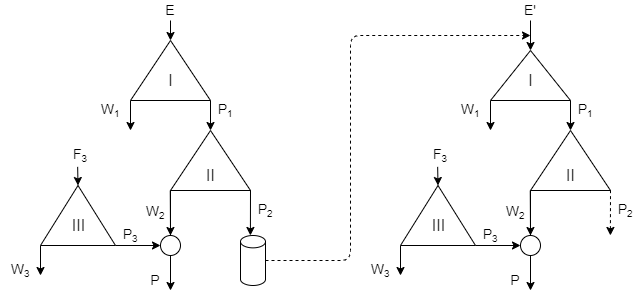
\includegraphics[scale=0.6]{cascades/P2utilizationRing}}
    \caption{Схема передачи загрязненной изотопом $^{232}$U фракции гексафторида урана в двойном каскаде от первой партии дообогащенного регенерированного урана к последующей. Обозначения: $E$ -- поток регенерированного урана; $P_1$ -- поток отбора первого каскада, выступающий питанием второго каскада; $P_2$ -- поток отбора второго каскада; $W_1$ -- поток отвала первого каскада; $W_2$ -- поток тяжелой фракции (условный «отвал») второго каскада; $P_0$ -- поток НОУ-разбавителя; $P$ -- финальный продукт (товарный низкообогащенный уран (НОУ), который подается на питание последующего двойного каскада, перемешиваясь с регенератом очередного рецикла}\label{P2utilizationRing}
\end{figure}

Учитывая, что каскадная схема двойного каскада с НОУ-разбавителем (рис. \ref{p2left}) предназначена для обогащения регенерата с высоким накопившимся в ходе серии пройденных рециклов содержанием изотопа $^{232}$U, можно использовать такую каскадную схему для вовлечения ранее полученного в потоке отбора второго каскада фракции $P_2$ загрязненной изотопом $^{232}$U. Выведенный ранее из системы гексафторида урана может быть перемешан с регенератом, полученным из следующей партии отработавшего топлива, то есть с составом более загрязненным изотопами $^{232,233,234,236}$U, чем исходно использовавшийся состав, побочным продуктом которого оказался этот $P_2$. Полученная таким образом в результате смешения $P_2$ предыдущего рецикла и регенерата очередного рецикла смесь будет отправлена на последующее обогащение (рис. \ref{P2utilizationRing}).

При использовании подобной схемы удастся полностью замкнуть топливный цикл по урану, а единственным отходом производства останется ОГФУ, образующийся в отвале первого каскада, который можно считать штатным отходом обогатительного производства с отработанными технологиями хранения и переработки. При этом после завершения производственного цикла останется невостребованным только тот объем обогащенного по изотопу $^{232}$U гексафторида урана (загрязненной фракции легкого конца второго каскада (рис. \ref{P2utilizationRing})), который будет образован после обогащения последней партии регенерата. Таким образом, предложенный подход к дообогащению регенерата урана позволяет организовать полный возврат регенерированного урана в топливный цикл в течение всего жизненного цикла задействованного урана.

При схожем наборе достоинств и недостатков схемы двойного каскада с НОУ-разбавителем с возвратом потока $P_2$ в цикл (рис. \ref{P2utilizationRing}), достоинством схемы с возвратом $P_2$ является более глубокая выработка потенциала делящегося $^{235}$U, накапливаемого совместно с изотопами $^{232,233,234}$U в загрязненной фракции второго каскада. Это позволяет добиваться меньших потерь $^{235}$U на всем жизненном цикле используемого урана.

\subsection{Пример топливного цикла, осуществляемого посредством двойного каскада с НОУ-разбавителем с возвратом потока $P_2$ в цикл}

Вычислительный эксперимент выполнялся исходя из следующих предположений.

Ординарный каскад, с помощью которого был обогащен регенерат первого рецикла, заменяется для последующих рециклов двойным каскадом ((рис. \ref{p2left}) и  полученная с его помощью партия последующего регенерата, произведенная после дообогащения регенерата первой партии регенерата (или регенерата, выделенного из первой выгруженной группы ТВС из реактора, работающего на РУТ-топливе первого рецикла) фракция, обогащенная по изотопу $^{232}$U и имеющая 20\% содержание изотопа $^{235}$U смешивается с регенератом, полученным после переработки второй партии ОТВС. Полученную смесь направляют на дообогащение (рис. \ref{P2utilizationRing}).


Результаты расчета параметров двойных каскадов для этого случая приведены в табл. \ref{vest2019_2}. В случае, когда возврата потока отбора не происходит, параметры топлива для всех перегрузок второго рецикла совпадают с параметрами первой перегрузки из табл. \ref{vest2019_2}, а изотопный состав урана, попадающего в отходы на каждой перегрузке, и его количество, совпадает с составом возвращаемой фракции первой перегрузки из табл. \ref{vest2019_2}.

\begin{table}
\begin{tabular}{|c|c|c|c|c|c|c|}
    \hline \multicolumn{1}{c|}{ Номер перегрузки } & \multicolumn{2}{|c|}{ Первая перегрузка } & \multicolumn{2}{c|}{ Вторая перегрузка } & \multicolumn{2}{|c}{ Третья перегрузка } \\
    \hline Обогащение, $\%$ & $4.95$ & $4.4$ & $4.95$ & $4.4$ & $4.95$ & $4.4$ \\
    Расх. пр. U, кг & $139802.03$ & $58291.31$ & $135568.06$ & $56351.24$ & $133649.39$ & $56868.39$ \\
    Расх. рег. U, кг & $20604.65$ & $9961.54$ & $20860.12$ & $10082.89$ & $20929.42$ & $10118.12$ \\
    Расх. РР, отн.ед. & $263368.8$ & $109887.15$ & $254313.79$ & $106009.0$ & $252276.2$ & $108260.45$ \\
    Масса $P_2$, кг & $255.47$ & $121.36$ & $324.77$ & $156.59$ & $329.34$ & $220.37$ \\
    \hline
    \end{tabular}
    $C_i$, \%
    \begin{tabular}{c|c|c|c|c|c|c|c}
    \hline${ }^{232} \mathrm{U}$ & $4.43 \times 10^{-7}$ & $4.34 \times 10^{-7}$ & $4.80 \times 10^{-7}$ & $4.85 \times 10^{-7}$ & $5.00 \times 10^{-7}$ & $4.92 \times 10^{-7}$ \\
    ${ }^{233} \mathrm{U}$ & $1.33 \times 10^{-6}$ & $1.32 \times 10^{-6}$ & $1.50 \times 10^{-6}$ & $1.51 \times 10^{-6}$ & $1.74 \times 10^{-6}$ & $1.50 \times 10^{-6}$ \\
    ${ }^{234} \mathrm{U}$ & $5.87 \times 10^{-2}$ & $5.40 \times 10^{-2}$ & $6.14 \times 10^{-2}$ & $5.68 \times 10^{-2}$ & $6.38 \times 10^{-2}$ & $5.63 \times 10^{-2}$ \\
    ${ }^{235} \mathrm{U}$ & $5.154$ & $4.607$ & $5.207$ & $4.658$ & $5.212$ & $4.634$ \\
    ${ }^{236} \mathrm{U}$ & $4.76 \times 10^{-1}$ & $4.91 \times 10^{-1}$ & $6.16 \times 10^{-1}$ & $6.14 \times 10^{-1}$ & $6.22 \times 10^{-1}$ & $5.61 \times 10^{-1}$ \\
    ${ }^{238} \mathrm{U}$ & Остальное & Остальное & Остальное & Остальное & Остальное & Остальное \\
    \hline \multicolumn{4}{|c|}{ Изотопный состав возврашаемой фракции, $\%$}
    \end{tabular}
    % $C_i$, \%
    \begin{tabular}{|c|c|c|c|c|c|c|}
    \hline ${ }^{232} \mathrm{U}$ & $1.64 \times 10^{-5}$ & $1.75 \times 10^{-5}$ & $2.32 \times 10^{-5}$ & $2.36 \times 10^{-5}$ & $2.57 \times 10^{-5}$ & $2.34 \times 10^{-5}$ \\
    ${ }^{233} \mathrm{U}$ & $3.98 \times 10^{-5}$ & $4.17 \times 10^{-5}$ & $5.16 \times 10^{-5}$ & $5.21 \times 10^{-5}$ & $5.49 \times 10^{-5}$ & $5.15 \times 10^{-5}$ \\
    ${ }^{234} \mathrm{U}$ & $5.88 \times 10^{-1}$ & $6.03 \times 10^{-1}$ & $6.78 \times 10^{-1}$ & $6.81 \times 10^{-1}$ & $6.96 \times 10^{-1}$ & $6.73 \times 10^{-1}$ \\
    ${ }^{235} \mathrm{U}$ & $20.00$ & $20.00$ & $20.00$ & $20.00$ & $20.00$ & $20.00$ \\
    ${ }^{236} \mathrm{U}$ & $7.11$ & $7.04$ & $6.54$ & $6.54$ & $6.46$ & $6.55$ \\
    ${ }^{238} \mathrm{U}$ & Остальное & Остальное & Остальное & Остальное & Остальное & Остальное \\
    \hline
    \end{tabular}
    \caption{Изотопные составы и расходы природного урана для изготовления топлива для перегрузок реактора
    типа ВВЭР-1200 (без учета твэгов): топливо второго рецикла. Обозначения: $C_i$ -- изотопный состав возвращаемой фракции; Расх. РР, отн. ед. -- расход работы разделения в относительных единицах; пр. U -- природный уран; рег. U -- урановый регенерат}\label{vest2019_2}
\end{table}


Как видно из данных табл. \ref{vest2019_2} предложенная схема рециклирования действительно позволяет полностью израсходовать и исходный регенерированный уран и образующийся в результате использования двойного каскада высокообогащенный отход.

Итак, опираясь на результаты расчетов, можно сделать общие выводы касаемо двойного каскада с НОУ-разбавителем с возвратом потока $P_2$ в цикл:

\begin{enumerate}
    \item схема принципиально применима для обогащения регенерированного урана в условиях многократного рецикла урана в топливе легководных реакторов, поскольку позволяет получать продукт, отвечающий всем требованиям по концентрациям четных изотопов для регенерата различного исходного состава;
    \item достоинством схемы является полное отсутствие потерь $^{235}$U (не считая потока отвала первого каскада) в процессе рециклирования, а также полное отсутствие нештатного отхода вплоть до последней перегрузки последнего рецикла; Однако, ввиду искусственного повышения содержания четных изотопов $^{232,234}$U в получаемом продукте с каждой последующей перегрузкой возрастает масса отхода  $P_2$ и, соответственно, масса концентрирующегося в нем изотопа $^{235}$U, что уменьшает эффект от возврата изотопа $^{235}$U в цикл из-за его потерь вследствие увеличения потока загрязненной фракции, которое происходит вследствие роста концентраций четных изотопов в исходной смеси.
    \item возврат фракции отхода (потока $P_2$) в схему является причиной монотонного роста концентраций четных изотопов, что приводит к необходимости увеличения уровня обогащения получаемого НОУ и, тем самым, к росту затрат работы разделения, а также повышению концентрации изотопа $^{235}$U в НОУ-разбавителе ввиду необходимости компенсации влияния $^{236}$U;
    \item в схеме присутствуют потери работы разделения из-за необходимости обеднять отбор второго ординарного каскада $P_2$ в последующей составной каскадной схеме;
\end{enumerate}


В качестве общего вывода по результатам анализа схемы двойного каскада с НОУ-разбавителем с возвратом $P_2$ в топливный цикл (рис. \ref{p2left}) представим следующее:
\begin{enumerate}
    \item схема применима для обогащения регенерированного урана в условиях многократного рецикла урана в топливе легководных реакторов, поскольку позволяет получать продукт, отвечающий всем требованиям на концентрации четных изотопов на основе состава регенерата с повышенным исходным содержанием изотопов $^{232,234}$U, который не позволяет решить проблему с помощью ординарного каскада;
    \item схема позволяет использовать поток «легкой» фракции второго каскада ($P_2$), поскольку указанный поток возвращается в топливный цикл, что снимает проблемы его долговременного хранения и связанные с ним затраты;
    \item схема c возвратом $P_2$ как и предшествующая схема без возврата $P_2$, подходит для решения задачи обогащения урана при одновременном выполнении всех сопутствующих условий, в том числе, при обогащении регенерированного урана, прошедшего несколько последовательных рециклов;
    \item схема c возвратом $P_2$ как и предшествующая схема двойного каскада с НОУ-разбавителем, позволяет задействовать для воспроизводства ядерного топлива накопленный в значительных количествах обедненный уран. Производимый ею отвал регенерированного урана ($W_1$) имеет содержание четных изотопов на уровне ниже допустимых ограничений. Это позволяет говорить о том, что такие отвалы могут безопасно длительно хранится в виде гексафторида урана или быть переработанными на установке дефторирования;
    \item в схеме на трех стадиях процесса обогащения происходят потери работы разделения:
    \begin{enumerate}
        \item обеднение отбора первого каскада $P_1$ во втором каскаде;
        \item смешивание потоков $W_2$ с НОУ-разбавителем $P_0$, в которых различается содержание изотопа $^{235}$U;
        \item смешивания потоков $P_2$ и $E$ на входе в каскады, принимающие регенерат последующих рециклов (начиная с третьего).
    \end{enumerate}
    \item в схеме, как и в предшествующей немодифицированной схеме двойного каскада с НОУ-разбавителем, физически разделены участки каскада с разделительным оборудованием, пропускающие через себя регенерированный урана (первые два каскады, принимающие на вход поток $E$ на рисунке \ref{P2utilizationRing}) и участок обогащения сырья для наработки НОУ-разбавителя -- природного или обедненного урана -- материалов, которые не загрязнены четными изотопами $^{232,236}$U. В дальнейшем это позволит задействовать оборудование каскада, использовавшегося для наработки разбавителя, в операциях обогащения природного урана или другого сырьевого материала, не загрязненного четными изотопами, а значит в менее жестконормированных условиях эксплуатации;
    \item практическая реализация представляется нецелесообразной, поскольку данная схема не дает ощутимых преимуществ с точки зрения интегральной экономии $^{235}$U в топливном цикле по отношению к схеме двойного каскада с НОУ-разбавителем (рис. \ref{p2left}), причем реализации схемы с возвратом $P_2$ возможна только в условиях непрерывной работы реактора и постоянного поступления новых партий регенерата на дообогащение.
\end{enumerate}


\subsection{Пример замыкания для утилизации отходов очистки регенерата урана от четных изотопов в двойном каскаде}

Процесс возврата данного материала в воспроизводство низкообогащенного урана может быть начат также и после дообогащения регенерата уже для одной ТВС и даже для ее части (непрерывный возврат), схема каскада при этом преобразуется к виду, изображенному на рис. \ref{net}. 

\begin{figure}[ht]
    \centerfloat{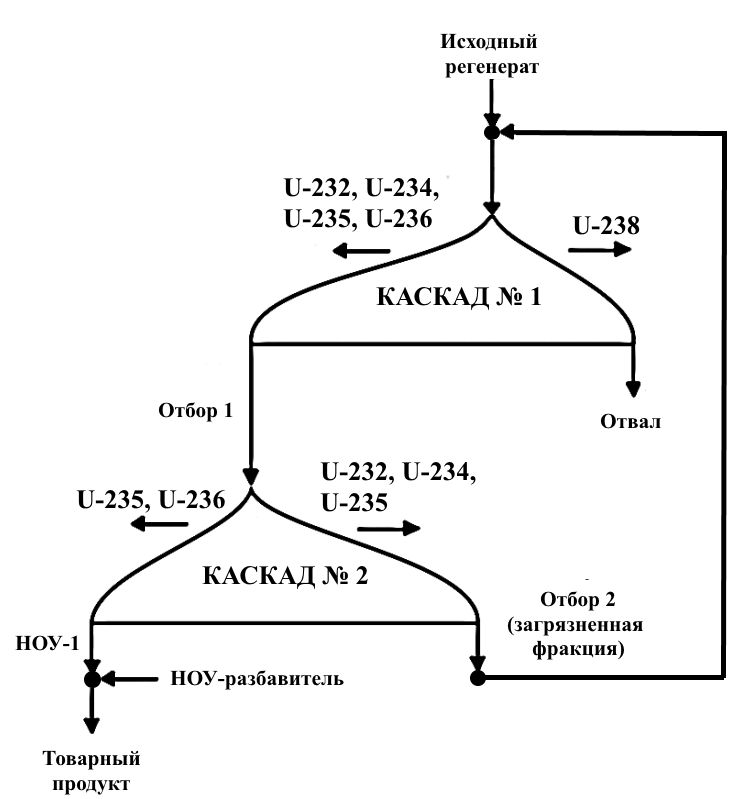
\includegraphics[scale=0.5]{cascades/net}}
    \caption{Схема двойного каскада с возвратом потока отбора.}\label{net}
\end{figure}


Очевидно, что при использовании предлагаемой схемы и непрерывной работе завода по обогащению, удастся полностью замкнуть топливный цикл по урану, а единственным отходом производства станет только обедненный гексафторид, образующийся в отвале первого каскада. Однако данный продукт можно считать штатным отходом обогатительного производства, для которого на сегодняшний день отработаны технологии хранения и переработки. При этом после вывода завода из эксплуатации (или остановки на планово-предупредительный ремонт) останется невостребованным только тот объем обогащенного по изотопу $^{232}$U гексафторида урана, который будет образован после обогащения последней партии регенерата на этом заводе. Таким образом, рассматриваемый подход к дообогащению регенерата урана позволяет организовать полный возврат регенерированного урана в топливный цикл в течение практически всего жизненного цикла топлива легководных реакторов, работающих в замкнутом топливном цикле.

Несмотря на очевидные достоинства рассматриваемого способа, возникает вопрос о его эффективности с точки зрения интегральных характеристик разделительного каскада, важных для экономики топливного цикла в целом. Речь идет об экономии природного урана в цикле и затратах работы разделения на единицу массы готового НОУ.
В связи с этим целью настоящей работы явилась оценка интегральных показателей для рассматриваемой схемы в условиях ее использования для обогащения регенерированного урана и наработки НОУ для обеспечения поставок для формирования топлива нескольких последовательных загрузок реактора.

Исходный регенерат второго рецикла использован для производства тепловыделяющих сборок (ТВС) c обогащением: 4,95\%. Из указанного состава изготавливают сначала топливо для первой перегрузки. Далее, загрязненную фракцию от обогащения регенерата для первой перегрузки перемешивают с регенератом исходного состава для второго рецикла и направляют на последующее обогащение для получения топлива следующей перегрузки. Всего рассмотрено 7 перегрузок. При расчете состава низкообогащенного урана после каскада при получении топлива для каждой из перегрузок решается оптимизационную задачу (метод прямого поиска) для шести выбранных критериев эффективности при шаге по концентрации в потоке отбора первого каскада и потоках отбора и отвала второго каскада равном 1\%. Для сопоставления отбирали только те варианты, для которых выполнены описанные выше условия для концентраций четных изотопов. Диапазоны варьирования концентраций в выходящих потоках каскадной схемы были следующими. Концентрацию $^{235}$U в первом каскаде варьировали в диапазоне 7-17\%, в отвале второго каскада 6-16\%, в отборе второго каскада 10-20\%.

Ввиду сложности многокритериального анализа для каждой из перегрузок был рассмотрен случай с параллельными «ветками», на каждой из которых проводили последовательный расчет изотопных составов и параметров разделительного каскада для семи перегрузок, при условии оптимизации на каждом из шагов по одному и тому же критерию эффективности. В качестве критериев эффективности выступали величины: (1) минимум расхода природного урана на единицу продукта, (2) минимум затрат работы разделения на единицу продукта, (3) минимум концентрации изотопа $^{232}$U (в диапазоне 2-$5\cdot10^{-7}$\%), (4) минимум концентрации изотопа $^{236}$U, (5) минимум массы отхода двойного каскада, (6) максимум степени извлечения $^{235}$U из поступающего в обогащение регенерата. Под степенью извлечения $^{235}$U из исходного регенерированного урана понимали отношение массы $^{235}$U в отвале второго каскада к массе $^{235}$U в исходной смеси регенерата, поступившего для обогащения.

Далее представлены результаты проведенных вычислительных экспериментов и проведен их анализ. 
На рисунке \ref{3} представлено изменение удельного расхода природного урана при получении товарного НОУ при шести различных критериях эффективности, по которым осуществляли оптимизацию для каждой перегрузки. Как следует из анализа зависимостей, показанных на указанном рисунке при оптимизации по четырем, а именно: минимуму удельного расхода природного урана, минимуму удельных затрат работы разделения, минимуму массы отхода двойного каскада, максимуму степени извлечения $^{235}$U из поступающего в обогащение регенерата, зависимости практически совпадают. Это можно объяснить тем, что данные критерии близки по своей сути. Например, максимум степени извлечения $^{235}$U из поступающего в обогащение регенерата должен приводить к необходимости использования минимальной массы $^{235}$U из природного сырья, что и выражается в уменьшении расхода природного сырья. В целом все кривые представляют собой уменьшающиеся функции, что логично, учитывая, что с каждой перегрузкой масса исходного регенерата возрастает одновременно с повышением концентрации $^{235}$U в нем. Однако при использовании в качестве критериев эффективности минимумов концентраций $^{232}$U и $^{236}$U в товарном НОУ соответствующие кривые заметно отличаются от четырех упомянутых выше случаев. Как можно видеть из рисунка \ref{3} (кривые 4 и 5) для этих случаев характерен заметно больший расход природного урана. Данный факт можно объяснить тем, что при оптимизации по минимуму концентраций четных изотопов в товарном НОУ происходит «вытеснение» четных изотопов, а вместе с ними и значительной массы $^{235}$U в отбор второго каскада. В результате заметно падает степень извлечения $^{235}$U из исходного регенерата (рисунок \ref{4}) и масса отхода, что отчетливо заметно по зависимостям на рисунке \ref{5}, в соответствии с которыми масса отхода для этих критериев на последних перегрузках превышает массу исходного регенерата и составляет величину более 30\% от массы исходного регенерата. В то время как для других критериев эта величина даже на 7-й перегрузке не превышает 10\%. Общей закономерностью для всех случаев является снижение расхода природного сырья с каждой перегрузкой (рисунок \ref{6}).


\begin{figure}[ht]
    \begin{minipage}{.5\textwidth}
      \centering
      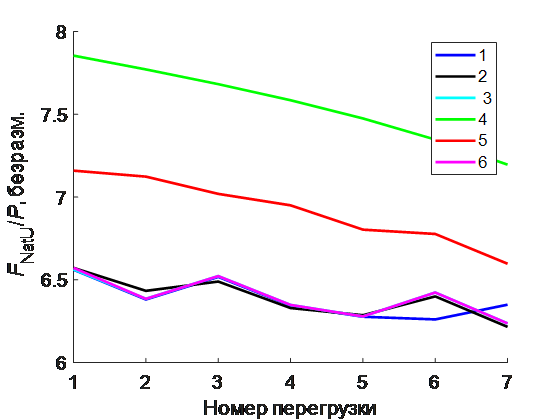
\includegraphics[width=.8\linewidth]{images/net/3}  
      \caption{Изменение величины удельного расхода природного урана в двойном каскаде с замыканием в зависимости от номера перегрузки для обогащения 4,95\% для различных критериев эффективности.}
      \label{3}
    \end{minipage}
    \begin{minipage}{.5\textwidth}
      \centering
      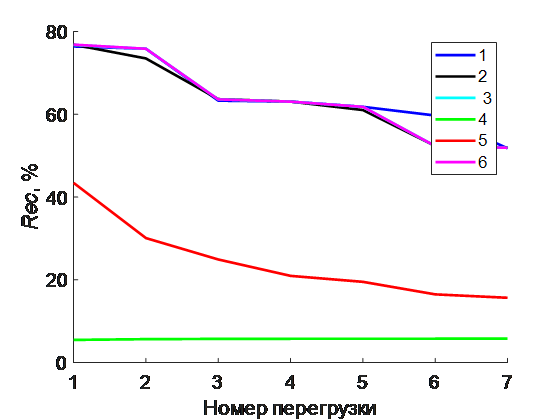
\includegraphics[width=.8\linewidth]{images/net/4}  
      \caption{Степень извлечения $^{235}$U из исходного регенерата в зависимости от номера перегрузки для обогащения 4,95\% для различных критериев эффективности.}
      \label{4}
    \end{minipage}
    \begin{minipage}{.5\textwidth}
      \centering
      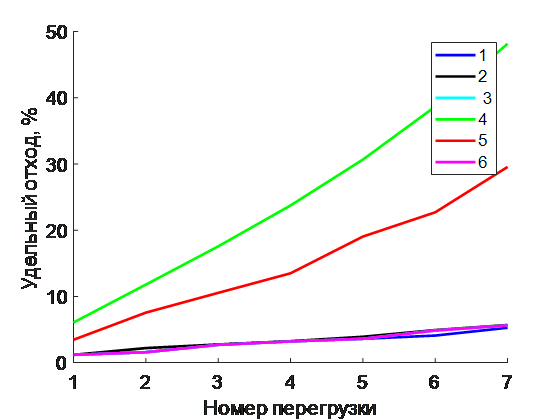
\includegraphics[width=.8\linewidth]{images/net/5}  
      \caption{Величину удельного отхода (на единицу исходного регенерата) в зависимости от номера перегрузки для обогащения 4,95\% для различных критериев эффективности.}
      \label{5}
    \end{minipage}
    \begin{minipage}{.5\textwidth}
      \centering
      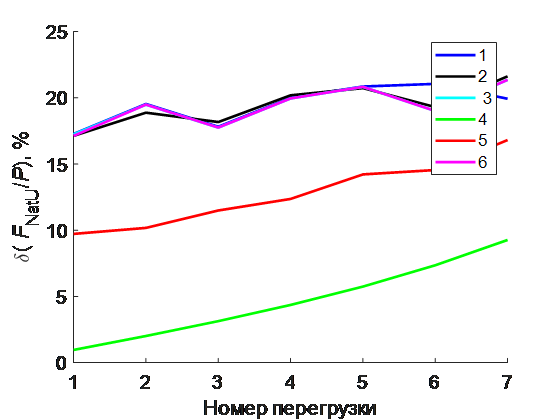
\includegraphics[width=.8\linewidth]{images/net/6}  
      \caption{Относительное изменение величины удельного расхода природного урана в двойном каскаде с замыканием в зависимости от номера перегрузки для обогащения 4,95\% для различных критериев эффективности.}
      \label{6}
    \end{minipage}
\end{figure}


Обозначения для рис. \ref{3}–\ref{6} приняты следующие. Кривая 1: оптимумы по расходу природного урана, кривая 2: оптимумы по затратам работы разделения, кривая 3: оптимумы по массе высокообогащенной фракции, кривая 4: минимум концентрации $^{232}$U, кривая 5: минимум концентрации $^{236}$U, кривая 6: максимум степени извлечения минимум $^{235}$U из регенерата урана.

В результате описанных выше процессов увеличивается и достигает значений, близких к 2, величина отношения (исходный регенерат)/продукт (риc. \ref{7}). Анализ зависимостей концентраций $^{235}$U и четных изотопов в регенерате, поступающем на обогащение после смешивания с высокообогащенной фракцией показывает, что все они повышается с каждой перегрузкой (рисунки \ref{8}–\ref{11}). Однако при использовании в качестве критериев эффективности минимумов концентраций  $^{232}$U и  $^{236}$U в товарном НОУ концентрации всех указанных выше изотопов в исходном регенерате возрастают заметно интенсивнее. Важно при этом отметить, что на последних перегрузках концентрация $^{235}$U в исходном регенерате превышает величину, требуемую для финального продукта (рисунок \ref{11}). Это означает, что схема начинает обеднять смесь и «чистить» ее от четных, а не обогащать. Особенно сильно это проявляется при минимизации концентраций четных изотопов в продукте, поскольку в этих случаях концентрация $^{235}$U в исходном регенерате могут приближаться к 5\% (рисунок \ref{10}). Подобные результаты говорят, в первую очередь, о нецелесообразности использования схемы в таком варианте для последовательного обогащения регенерата нескольких перегрузок с использованием в качестве критериев эффективности на каждом шаге требования минимальности концентраций $^{232}$U и  $^{236}$U в товарном НОУ. Однако требуют дополнительных исследований возможности дальнейшей модификации предложенной схемы, в том числе, для более эффективного использования исходного регенерата с повышенным содержанием $^{235}$U. Одним из таких вариантов может стать расширение диапазона увеличения концентрации  $^{235}$U в схеме, например, до 90\%. Другие варианты могут быть основаны на введении дополнительных потоков для разбавления четных изотопов и снижения концентрации  $^{235}$U до нужных значений.

\begin{figure}[ht]
    \centerfloat{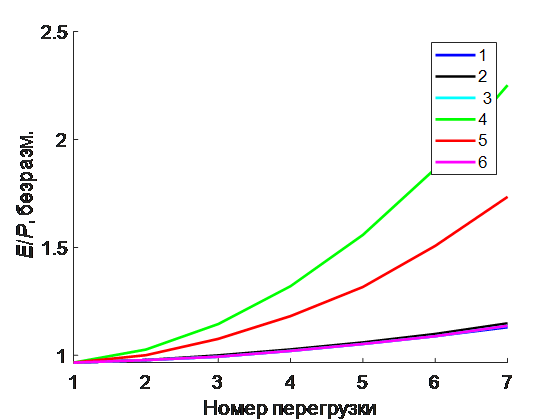
\includegraphics[scale=0.7]{images/net/7}}
    \caption{Зависимость отношения потоков исходного регенерата и финального продукта (товарного НОУ) от номера перегрузки для обогащения 4,95\% для различных критериев эффективности.}\label{7}
\end{figure}

\begin{figure}[ht]
    \begin{minipage}{.5\textwidth}
      \centering
      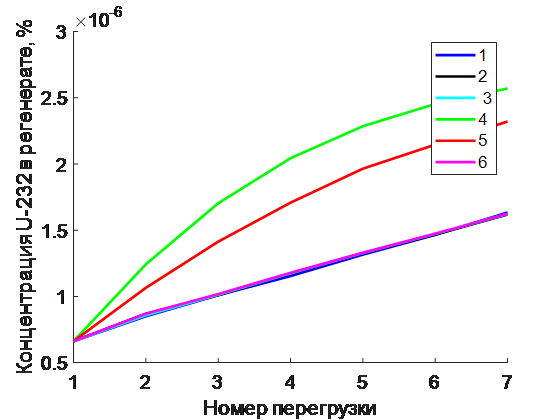
\includegraphics[width=.8\linewidth]{images/net/8}  
      \caption{Зависимость концентрации $^{232}$U в исходном регенерате от номера перегрузки для обогащения 4,95\% для различных критериев эффективности.}
      \label{8}
    \end{minipage}
    \begin{minipage}{.5\textwidth}
      \centering
      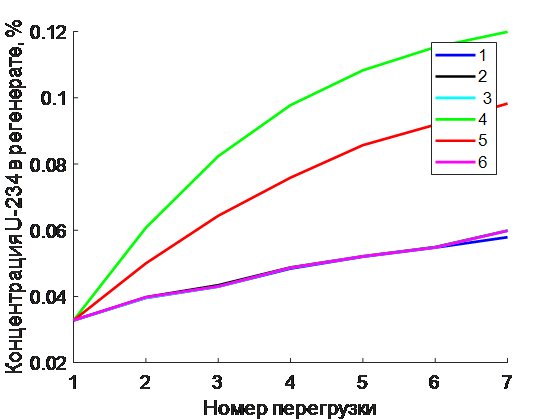
\includegraphics[width=.8\linewidth]{images/net/9}  
      \caption{Зависимость концентрации $^{234}$U в исходном регенерате от номера перегрузки для обогащения 4,95\% для различных критериев эффективности.}
      \label{9}
    \end{minipage}
    \begin{minipage}{.5\textwidth}
      \centering
      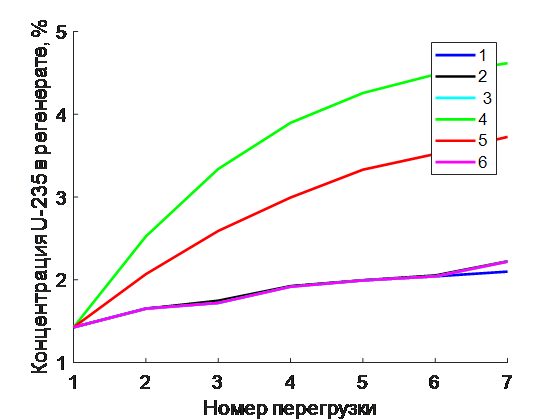
\includegraphics[width=.8\linewidth]{images/net/10}  
      \caption{Зависимость концентрации $^{235}$U в исходном регенерате от номера перегрузки для обогащения 4,95\% для различных критериев эффективности.}
      \label{10}
    \end{minipage}
    \begin{minipage}{.5\textwidth}
        \centering
        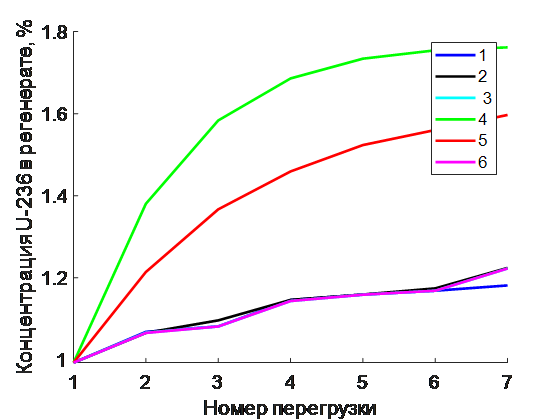
\includegraphics[width=.8\linewidth]{images/net/11}  
        \caption{Зависимость концентрации $^{236}$U в исходном регенерате от номера перегрузки для обогащения 4,95\% для различных критериев эффективности.}
        \label{11}
      \end{minipage}
\end{figure}

Обозначения для рис. \ref{7}–\ref{11} приняты следующие. Кривая 1: оптимумы по расходу природного урана, кривая 2: оптимумы по затратам работы разделения, кривая 3: оптимумы по массе высокообогащенной фракции, кривая 4: минимум концентрации $^{232}$U, кривая 5: минимум концентрации $^{236}$U, кривая 6: максимум степени извлечения минимум $^{235}$U из регенерата урана), E – поток питающего каскадную схему регенерата, P -- товарный НОУ.


Анализ изменения величины затрат работы разделения в зависимости от номера перегрузки и выбранного критерия эффективности показывает следующее. Для всех критериев, кроме случаев минимизации концентрации $^{232}$U или $^{236}$U затраты работы разделения сохраняются на определенном уровне, незначительно отличающемся от случая обогащения природного урана до соответствующей концентрации (рисунок \ref{12}). С увеличением номера перегрузки происходит незначительное снижение потерь работы разделения для этих случаев: с $\approx$5\% до $\approx$10\% (рисунок \ref{13}). При этом в случае минимизации концентраций изотопов $^{232}$U или $^{236}$U затраты работы разделения значительно выше и  могут на десятки процентов превосходить аналогичные затраты для случая обогащения природного урана для получения эквивалентного количества требуемого НОУ.

\begin{figure}[ht]
    \begin{minipage}{.5\textwidth}
      \centering
      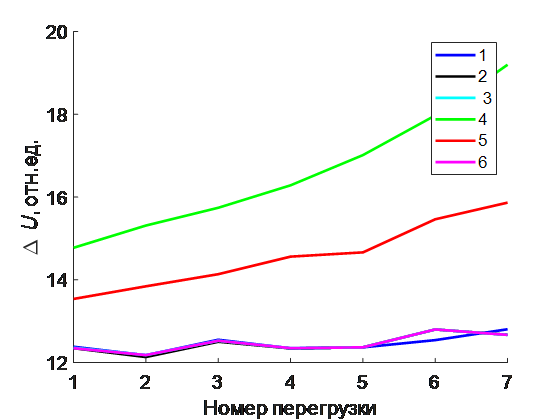
\includegraphics[width=.8\linewidth]{images/net/12}  
      \caption{Изменение величины удельных затрат работы разделения в двойном каскаде с замыканием в зависимости от номера перегрузки для обогащения 4,95\% для различных критериев эффективности.}
      \label{12}
    \end{minipage}
    \begin{minipage}{.5\textwidth}
      \centering
      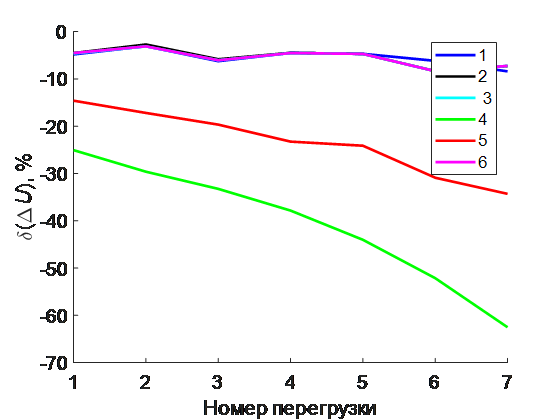
\includegraphics[width=.8\linewidth]{images/net/13}  
      \caption{Относительное изменение величины удельных затрат работы разделения в двойном каскаде с замыканием в зависимости от номера перегрузки для обогащения 4,95\% для различных критериев эффективности.}
      \label{13}
    \end{minipage}
\end{figure}

Обозначения для рис. \ref{12}–\ref{13} приняты следующие. Кривая 1: оптимумы по расходу природного урана, кривая 2: оптимумы по затратам работы разделения, кривая 3: оптимумы по массе высокообогащенной фракции, кривая 4: минимум концентрации $^{232}$U, кривая 5: минимум концентрации $^{236}$U, кривая 6: максимум степени извлечения минимум $^{235}$U из регенерата урана.

Рассматриваемая каскадная схема может работать в широком диапазоне изменения концентраций компонентов, в первую очередь, четных изотопов и $^{235}$U в исходном регенерате. Данный факт открывает возможности для применения схемы в условиях топливных циклов с увеличенной длительностью топливного цикла, а также в условиях многократного рецикла урана.

В зависимости от выбранного критерия эффективности для оптимизации схемы при расчете изотопного состава НОУ для каждой новой перегрузки, возможно обеспечить широкую вариативность параметров рассматриваемой каскадной схемы. При этом в случае выбора в качестве критериев эффективности величин удельного расхода природного урана, удельных затрат работы разделения, массы получаемого отхода или величины степени извлечения $^{235}$U из исходного регенерата оптимальные параметры схемы меняются незначительно. В то время, как при использовании в качестве критериев эффективности условий минимума концентраций $^{232}$U и $^{236}$U в товарном НОУ ключевые характеристики каскадов значительно отличаются от других критериев.

С ростом номера перегрузки происходит последовательно уменьшение расхода природного урана и затрат работы разделения. При этом на последних перегрузках экономия природного урана достигает величины 20\% и более. Это означает, что экономия природного урана в цикле в среднем будет примерно на треть выше типичного значения в 15\%. Причиной этому более эффективное использование $^{235}$U из регенерата.







\section{Схема тройного каскада с НОУ-разбавителем и дополнительным разбавителем потока $P_2$, возвращаемого в цикл}

Другим способом утилизации загрязненной фракции стала схема тройного каскада \cite{smirnovApplyingEnrichmentCapacities2018}. Принцип ее работы состоит в следующем.

\begin{figure}[ht]
    \centerfloat{
\includegraphics[scale=0.9]{cascades/p2_withDepU}}
    \caption{Тройной каскад для обогащения регенерированного урана. Обозначения: $E$ -- поток регенерированного урана; $P_1$ -- поток отбора первого каскада, выступающий питанием второго каскада; $P_2$ -- поток отбора второго каскада; $F_{du}$ -- поток ОГФУ-разбавителя, смешиваемого с $P_2$ перед подачей на вход третьего каскада; $W_1$ -- поток отвала первого каскада; $W_2$ -- поток тяжелой фракции (условный «отвал») второго каскада; $P_0$ -- поток НОУ-разбавителя; $P$ -- финальный продукт (товарный низкообогащенный уран (НОУ)), полученный смешиванием потоков $W_2$, $P_0$ и $P_3$, где $P_3$ -- отбор третьего каскада; $W_3$ -- отвал третьего каскада.}\label{p2_withDepU}
\end{figure}

В реализации такой схемы поток легкой фракции второго каскада $P_2$ c концентрацией изотопа $^{235}$U на уровне 20\% перемешивается со складским ОГФУ и направляется на последующее обогащение в третий каскад (рис. \ref{p2_withDepU}). Пропорцию смешивания $P_2$ с ОГФУ определяют исходя из возможности получить НОУ надлежащего качества при обогащении их смеси (оставаясь в рамках ограничений по четным изотопам). Остальные параметры схемы тройного каскада следует подбирать исходя из того, что финальный продукт будет получен смешиванием трех потоков: низкообогащенного <<чистого>> разбавителя $P_0$, тяжелой <<очищенной>> фракции $W_2$ второго каскада и, полученного при обогащении потока $P_2$ и обедненного урана, изотопного состава $P_3$. Управляющими параметрами являются: концентрации на выходах $P_1$ первого и $P_2$ второго каскадов, а также в потоке НОУ-разбавителя $P_0$. При детерминированной их комбинации обеспечивается соответствие предзаданному отношению масс конечного продукта и исходного регенерата, за счет чего выполняется условие полного возврата. При этом проблема высокоактивного отхода решается без выхода за пределы концентрации допустимой для обогащения регенерата (20\%). Также устраняется необходимость обращения с $P_2$, которое в схеме двойного каскада с НОУ-разбавителем с возвратом потока $P_2$ в цикл (рис. \ref{P2utilizationRing}) связано с его отложенным вовлечением из-за зависимости от последующих поступлений на обогащение новых партий (последующих рециклов) регенерата.

Таким образом, решение проблемы накопления нештатного отхода, характерной для двойного каскада с НОУ-разбавителем, состоит в том, что поток легкой фракции второго каскада ($P_2$) перемешивают с обедненным ураном и направляют на последующее обогащение в еще один каскад (крайний правый каскад на рисунке \ref{p2_withDepU}).


Для расчета двойного каскада с НОУ-разбавителем, результатом которого будет нахождение параметров схемы, необходимых для задания при требуемых концентрациях в выходных потоках, выбираются переменные $C_{W_2}^{235}$ и $C_{P_0}^{235}$ при невязках, связанными с достижением требуемой концентрации $^{235}$U в продукте, с учетом поправки на $^{236}$U: $C_{235 экв.}^{P}=C_{235 прир.}^{P}+\Delta C_{235}$, а также с выполнением ограничения на концентрацию $^{232}$U, задавая содержание этого изотопа в продукте равным предельно допустимому значению, что необходимо для решения получившейся системы нелинейных уравнений (СНАУ). Такая постановка задачи, реализованная, например, в \cite{gusevMultycascadeEnrichmentSchemes2020}, позволила показать возможность решения задачи возврата регенерата в цикл для состава пятого рецикла при заданной пропорции регенерата к конечному продукту, соответствующей использованию всего выделенного из ОЯТ урана. Как показывают результаты анализа повторного обогащения регенерата пятого рецикла с помощью такой схемы, это операция ценой расхода дополнительных 25\% работы разделения, удается вернуть заданное количество переработанного урана, прошедшего пятикратное (5 топливных кампаний) облучение, сэкономив $\approx$15\% природного урана, сравнивая приведенные показатели со схемой ординарного каскада для обогащения природного урана, получающего на выходах в продукте и отвале такие же концентрации $^{235}$U (соответствующую $C_{235 экв.}$ в продукте). В другом варианте реализации схемыценой расхода дополнительных 25\% работы разделения, удается вернуть заданное количество переработанного урана, прошедшего пятикратное (5 топливных кампаний) облучение, сэкономив $\approx$15\% природного урана, сравнивая приведенные показатели со схемой ординарного каскада для обогащения природного урана, получающего на выходах в продукте и отвале такие же концентрации $^{235}$U (соответствующую $C_{235 экв.}$ в продукте) тройного каскада ценой расхода дополнительных 50\% работы разделения, удается вернуть заданное количество переработанного урана, прошедшего пятикратное (5 топливных кампаний) облучение, сэкономив $\approx$23\% природного урана \cite{gusevMultycascadeEnrichmentSchemes2020}.


Для анализа возможностей схемы тройного каскада с НОУ-разбавителем, представим расчет, оценивающий издержки ее применения для возврата регенерата пятого рецикла. 
В качестве ключевых оцениваемых характеристик будем опираться на экономию природного урана, а также долю дополнительно задействуемых в каскаде центрифуг, по сравнению с ординарным каскадом для обогащения природного урана. Проведем сравнение со схемой с разбавлением регенерата природным ураном перед подачей в ординарный трехпоточный каскад \ref{o3} \cite{smirnovMethodEnrichReprocessed2019}. Обе сравниваемые схемы должны обеспечить производство НОУ коммерческого качества, то есть удовлетворяющего всем заданным условиям.

В таблице \ref{tr_ch} представлены величина экономии природного урана, потребление регенерированного урана на единицу продукта, а также количество центрифуг для предложенной трехкаскадной схемы и модифицированного ординарного каскада, по сравнению с базовым вариантом -- ординарным  каскадом, обогащающим природный уран. Количество центрифуг для всех вариантов приводится к количеству центрифуг в ординарном каскаде для обогащения природного урана.

\begin{table}[h]
\centering
\normalsize\begin{tabulary}{1.0\textwidth}{CCCCCCC}
    Каскад & Экономия природного урана, \% & Доп. разделительные мощности, \% & Расход регенерата на ед. продукта \\
    Ординарный модифицированный & 7.1 & 3.6 & 49.2 \\
        &  &  &   \\
    Двойной каскад с НОУ-разбавителем & 38.3 & 97.3 &  92.4 \\
        &  &  &   \\
\end{tabulary}
\caption{{Оцениваемые параметры рассматриваемых схем{\label{tr_ch}}}}
\end{table}

В табл. \ref{tr_prod} показан изотопный состав НОУ коммерческого уровня, полученного в предлагаемом тройном каскаде.

\begin{table}[h]
    \centering
    \normalsize\begin{tabulary}{1.0\textwidth}{ccccccc}
        Массовое число & 232 & 233 & 234 & 235 & 236 \\
        C, \% & 5.00e-7 & 6.88e-7 & 5.31e-2 & 5.11 & 0.57 \\
    \end{tabulary}
    \caption{{Изотопный состав НОУ-продукта схемы двойного каскада с НОУ-разбавителем и дополнительным разбавителем потока $P_2$, возвращаемого в цикл{\label{tr_prod}}}}
    \end{table}

Эти результаты показывают, что предложенная схема решает поставленную задачу. Сравнение с ординарным каскадом показывает, что даже при выбранном «грязном» составе регенерированного урана -- составе пятого рецикла -- можно сэкономить более трети природного урана, что намного больше, чем достижимо при использовании более простых модификаций. Однако, такие преимущества влекут за собой увеличение затрат разделительной работы, а следовательно, и количества центрифуг по сравнению с ординарным трехпоточным каскадом, который обогащает природный уран (примерно на 97\%). Схема также позволяет производить НОУ товарного качества, расходуя заранее определенное количество переработанного урана без нежелательных нештатных побочных продуктов, за исключением стандартных т.н. хвостов разделительного производства (потоков отходов) разделительных каскадов в виде обедненного урана.

Рассчитывая материальные балансы в этой схеме, исходя из предположения, что будет произведена ровно 21 тонна НОУ. Примерно такая масса урана требуется для загрузки реактора ВВЭР-1200 твэлами с обогащением 4,95\%. Имея заданное отношение регенерата к конечному продукте 0,93, регенерированный уран будет израсходован из расчета 19,53 тонны на 21 тонну конечного продукта НОУ. В нашем случае первый каскад производит 17,5 т обедненного урана в потоке $W_1$, что дает $\approx$2,03 т $P_1$ с концентрацией $^{235}$U, равной 9,41\%. Поток $P_1$ запитывает второй каскад, который, в свою очередь, производит «очищенную» смесь $W_2$ (1,7 тонны, которая содержит 7,34\% $^{235}$U) и загрязненный $P_2$ ($\approx$332 кг), который содержит 20\% $^{235}$U. $P_2$ поступает в третий каскад и там разбавляется 3298,88 т. обедненного урана с концентрацией $^{235}$U 0,1\%. В третьем каскаде обедняющая часть состоит всего из 1 ступени, выдает $\approx$3293,1 тонны отходов $W_3$  с 0,093\% $^{235}$U. НОУ-разбавитель $P_0$ $\approx$13,2 тонны смешивается с 1,7 тоннами $W_2$, образуя $\approx$14,9 тонны материала, которые затем, смешавшись с 6,1 тонны $P_3$, образуют 21 тонну конечного НОУ-продукта. Каскад, производящий НОУ-разбавитель $P_0$ (с концентрацией $^{235}$U 4,9\%), потребляет $\approx$103,6 тонны природного урана, отправляя в отвал $W_0$ 90,4 тонны (с концентрацией 0,1\% $^{235}$U). В результате схема производит (90,4 + 17,5 + 3293) $\approx$3401 тонну обедненного урана. При этом на схему уходит $\approx$3300 тонн складских запасов обедненного урана. Следовательно, фактический выход обедненного урана составляет $\approx$100 тонн, при том что ординарный каскад для обогащения природного урана при производстве такого же количества продукта (21 тонна) производит $\approx$146 тонн, то есть схема тройного каскада с НОУ-разбавителем и дополнительным разбавителем потока $P_2$, возвращаемого в цикл позволяет в полтора раза уменьшить накопление ОГФУ.

Также была предложена реализация поставленной задачи с помощью рассматриваемой схемы, в \cite{gusevMultycascadeEnrichmentSchemes2020}, демонстрирующей споcоб решения задачи возврата регенерата в цикл для состава пятого рецикла при заданной пропорции регенерата к конечному продукту, соответствующей использованию всего выделенного из ОЯТ урана, а также исключающий накопление нештатного отхода за счет разбавления $P_2$ обедненным гексафторидом с последующим обогащением. Как показывают результаты анализа повторного обогащения регенерата пятого рецикла с помощью такой схемы, осуществлять такую операцию можно с различными показателями затрат работы разделения, экономии природного урана, а также вовлечения ОГФУ. Например, ценой расхода дополнительных $\approx$25\% работы разделения, удается вернуть заданное количество переработанного урана, прошедшего пятикратное (5 топливных кампаний) облучение, сэкономив $\approx$15\% природного урана, при этом вовлекая в производство единицы конечного продукта $\approx$31 единицы смеси обедненного урана. Для экономии же природного урана на уровне $\approx$23\%, необходимо, использовав $\approx$74,5 единиц ОГФУ на единицу продукта, допустив перерасход работы разделения на уровне $\approx$50\%. Показатели приведены в соотношении с аналогичными для схемы ординарного каскада для обогащения природного урана, получающего на выходах в продукте и отвале такие же концентрации $^{235}$U (соответствующую $C_{235 экв.}$ в продукте).


Стоит отметить, что представленные примеры приведены только в иллюстративных целях. Чтобы применить эту схему на практике, в первую очередь необходимо оптимизировать ее по выбранному критерию эффективности.

Рассматривая возможность постановки оптимизационной задачи для тройного каскада, в качестве управляющих оптимизационных переменных можно рассматривать: концентрации $^{235}$U в потоках $P_1$, $P_2$ и $W_3$ и отношение потоков $F_{du}$/$P_2$.
Цель решения оптимизационной задачи: при заданных внешних условиях и выполнении заданных ограничений определить наилучшее значение критерия эффективности -- расхода работы разделения каскадной схемы, в зависимости от варьируемых переменных.

Также, помимо минимума расхода работы разделения, оптимизационным критерием может выступать минимизация расхода природного урана, а также максимум суммарной степени извлечения $^{235}$U в схеме \ref{Rec3} и из регенерата \ref{RecR3} для тройного каскада, где $RepU$ -- это поток регенерата, а $DepU_{3}$ -- поток разбавляющего $P_2$ ОГФУ.


\begin{equation} \label{Rec3} 
    U^{235}_{Rec} = \frac{LEU Product \cdot C_np}{F_0 \cdot C_{NatU}^{235} + RepU \cdot C_{RepU}^{235} + {DepU}_3 \cdot C_{DepU}^{235}}, 
\end{equation} 
\begin{equation} \label{RecR3} 
    RepU^{235}_{Rec} = \frac{W_2\cdot C_{W_2}^{235}+P_3\cdot C_{P_3}^{235}\cdot \frac{P_2\cdot C_{P_2}^{235}}{P_2\cdot C_{P_2}^{235}+ {DepU}_3 \cdot C_{DepU}^{235}}}{RepU \cdot C_{RepU}^{235}}        
\end{equation} 

Такой тип оптимизационной задачи также как и для предыдущих составных схем представляет собой задачу условной оптимизации функции многих переменных. В диссертационной работе предложена оригинальная методика, основанная на использовании современных методов условной оптимизации и реализованная в виде разработанного программного кода.
Следует отметить, что в литературе по данной тематике отсутствуют методики оптимизации трех- и четырехкаскадных схем в случае разделения многокомпонентных смесей. Фактически подобные задачи решены впервые.



\subsubsection{Оптимизация схемы тройного каскада с НОУ-разбавителем при различных критериях}

Рассмотрим предложенный в данной работе алгоритм подбора параметров каскадной схемы, который позволяет осуществить расчет двойного каскада с НОУ-разбавителем.

\begin{enumerate}
    \item варьируется (с шагом в 1\%) концентрация $^{235}$U, задаваемая в потоке отбора $P_2$ второго каскада. В качестве начальной точки задается значение 7\%, а финальной -- верхний порог ограничения ан обогащение $^{235}$U: 20\% или 90\%;
    \item внутри приведенного выше цикла со счётчиком, в котором переменная концентрации $^{235}$U изменяет своё значение от заданного начального значения (7\%) до конечного значения (20\% или 90\%) с шагом 1\%, для каждого значения этой выполняется тело цикла, в котором осуществляется подбор концентрации $^{235}$U в потоке отбора $P_1$ первого каскада. Они представляет собой цикл со счетчиком с шагом в 1\%, где варьируется концентрация $^{235}$U, задаваемая в потоке отбора $P_1$ первого каскада, начиная с 5\% до текущего значения концентрации $^{235}$U в $P_2$ минус 2\%.
    \item при определенных этими двумя циклами (варьирования $^{235}$U в $P_2$ и вложенным циклом варьирования $^{235}$U в $P_1$) концентрациях $^{235}$U в потоках отбора первого и второго каскада, осуществляется расчет системы нелинейных алгебраических уравнений с помощью вычислительного пакета MINPACK \cite{moreMINPACK}, переменными в которой выступают концентрации $^{235}$U в потоке отвала второго каскада, в потоке отбора третьего каскада, а также в потоке, полученном при смешении потоков $P_0$ и $W_2$  нарабатывающего НОУ-разбавитель. Невязками для этой системы служат расхождения, заданные условием задачи:
    \begin{enumerate}
        \item концентрации $^{235}$U в  конечном НОУ-продукте, с учетом поправки на $^{236}$U: $C_{235 экв.}^{P}=C_{235 прир.}^{P}+\Delta C_{235}$ от расчетного значения;
        \item концентрации $^{232}$U в конечном продукте от расчетного значения этой концентрации.
    \end{enumerate}
    При решении заданной СНАУ, сходимость достигается с помощью квазиньютоновского численного алгоритма trust-region, для которого якобиан вычисляется методом автодифференциации;
    \item для каждой итерации цикла со счетчиком выполняется оптимизационный алгоритм поиска глобального оптимума для заданного критерия эффективности, с помощью которого подбираются такие параметры схемы как: пропорция потока $P_2$ в питании третьего каскада; концентрации $^{235}$U в потоке отвала третьего каскада в интервалах [0.00001, 0.5] и [0.08\%, 0.13\%] соответственно. Для этого используется алгоритм оптимизации SHGO (simplicial homology global optimization) вычислительного пакета SciPy для Python  \cite{virtanenSciPyFundamentalAlgorithms2020a}.
    \item  на каждой итерации с помощью подбираемых значений переменных расчитываются основный параметры входящих в схему ординарных каскадов;
    \item  затем, на их основании необходимо расчитать пропорции потоков $W_2$, $P_3$ и $P_0$ в конечном продукте, для того чтобы получить массив значений изотопных концентраций для этого состава. Для этого, на основе вычисленных отношений потоков $\frac{P_{1}}{RepU}$, $\frac{W_{2}}{P_{1}}$ и $\frac{P_{3}}{F_{3}}$ для первого, второго и третьего каскадов, а также заданной условиями задачи пропорции $\frac{RepU}{P}$, где $RepU$ -- это поток регенерата, а $P$ -- поток финального НОУ-продукта, вычисляется необходимые параметры каскада;
    \item поочередно складывая покомпонентно умноженные доли $\frac{W_{2}}{P}$, $\frac{P_{3}}{P}$ и $\frac{P_{0}}{P}$ на соответствующие изотопные концентрации потоков $W_2$, $P_3$ и $P_0$, получается массив изотопных концентраций конечного НОУ-продукта. Для полученных в этом массиве значений концентраций $^{232}$U,$^{235}$U и $^{236}$U, расчитываются текущие величины расхождения (невязки) для двух равенств в СНАУ. Для каждой из них относительная ошибка (отклонение от единицы отношений левой и правой частей равенства) не должна превышать $10^{-8}$;
    \item соответствие выполненных условий для невязок означает схождение численного метода -- завершение вычислительных итераций и сохранением полученного решения для заданных внешними циклами значений концентраций $^{235}$U в $P_1$ и $P_2$, а также переменных (1) пропорция потока $P_2$ в питании третьего каскада и (2)концентрации $^{235}$U в потоке отвала третьего каскада, при которых достигается оптимум для заданного критерия;
    \item для полученного решения затем вычисляются основные характеристики схемы двойного каскада с НОУ-разбавителем, такие как расход работы разделения схемы или расход дополнительного сырья, которые позволяют оценить критерии эффективности каскадной схемы. Их значения также сохраняются для возможности последующего выбора решения исходя из выбора критерия эффективности.
\end{enumerate}



Для демонстрации возможностей, получаемых применением предложенных в диссертации методик оптимизации, представим серию расчетов тройного каскада с НОУ-разбавителем, получив интегральные показатели для различных оптимизационных критериев.


\begin{table}
    \begin{tabular}{ccccc}
        $\text{П-р | К-й опт-и}$ & $\text{max И}$ & $\text{max ИР}$ & $\text{min РР}$ & $\text{min NatU}$\\ \hline
        $\text{Сумм. степень изв-я}$ & $0.778$ & $0.07535$ & $0.07535$ & $0.03058$\\ \hline
        $\text{Степень изв-я из рег-та}$ & $0.7976$ & $0.8765$ & $0.8765$ & $0.7504$\\ \hline
        $\text{Потери РР, \%}$ & $6.814$ & $-1.127$ & $-1.127$ & $137.4$\\ \hline
        $\text{Расх. пр. U на ед. прод.}$ & $6.217$ & $6.246$ & $6.246$ & $0.922$\\ \hline
        $\text{Эк. пр. U, \%}$ & $21.62$ & $21.24$ & $21.24$ & $88.38$\\ \hline
        $\text{U-235 в P1, \%}$ & $5.0$ & $5.0$ & $5.0$ & $15.0$\\ \hline
        $\text{U-235 в W2, \%}$ & $4.227$ & $4.708$ & $4.708$ & $14.1$\\ \hline
        $\text{U-235 в P0, \%}$ & $5.425$ & $5.321$ & $5.321$ & $5.456$\\ \hline
        $\text{U-235 в P2, \%}$ & $16.0$ & $20.0$ & $20.0$ & $20.0$\\ \hline
        $\text{U-232 в P1, \%}$ & $2.443e-6$ & $2.443e-6$ & $2.443e-6$ & $7.431e-6$\\ \hline
        $\text{U-232 в W2, \%}$ & $1.515e-6$ & $1.998e-6$ & $1.998e-6$ & $6.329e-6$\\ \hline
        $\text{U-232 в P2, \%}$ & $1.564e-5$ & $2.526e-5$ & $2.526e-5$ & $1.357e-5$\\ \hline
        $\text{U-234 в P1, \%}$ & $0.1198$ & $0.1198$ & $0.1198$ & $0.3672$\\ \hline
        $\text{U-234 в W2, \%}$ & $0.09223$ & $0.1084$ & $0.1084$ & $0.3349$\\ \hline
        $\text{U-234 в P2, \%}$ & $0.512$ & $0.7049$ & $0.7049$ & $0.5472$\\ \hline
        $\text{U-236 в P1, \%}$ & $2.942$ & $2.942$ & $2.942$ & $6.159$\\ \hline
        $\text{U-236 в W2, \%}$ & $2.69$ & $2.856$ & $2.856$ & $5.955$\\ \hline
        $\text{Уд. сумм. поток к-а 2}$ & $6.009$ & $2.627$ & $2.627$ & $0.2777$\\ \hline
        $\text{Уд. сумм. поток доп. к-а}$ & $2285.0$ & $2285.0$ & $2285.0$ & $339.3$\\ \hline
        $\text{Доля P2 в F3}$ & $0.002519$ & $1.0e-5$ & $1.0e-5$ & $1.0e-5$\\ \hline
        $\text{U-235 в W3, \%}$ & $0.13$ & $0.13$ & $0.13$ & $0.1275$\\ \hline
        $\text{U-235 в P3, \%}$ & $5.319$ & $4.617$ & $4.617$ & $4.253$\\ \hline
        $\text{Р3, кг}$ & $74.86$ & $31.42$ & $31.42$ & $1219.0$\\ \hline
        $\text{U-232, \%}$ & $5.0e-7$ & $4.945e-7$ & $4.945e-7$ & $4.552e-7$\\ \hline
        $\text{U-234, \%}$ & $0.05795$ & $0.05973$ & $0.05973$ & $0.04356$\\ \hline
        $\text{U-235, \%}$ & $5.137$ & $5.155$ & $5.155$ & $5.072$\\ \hline
        $\text{U-236, \%}$ & $0.6463$ & $0.706$ & $0.706$ & $0.4194$\\ \hline
        $\text{P1, кг}$ & $372.8$ & $372.8$ & $372.8$ & $122.6$\\ \hline
        $\text{W2, кг}$ & $348.3$ & $365.6$ & $365.6$ & $103.9$\\ \hline
        $\text{P0, кг}$ & $1056.0$ & $1082.0$ & $1082.0$ & $155.7$\\ \hline
        $\text{Р2, кг}$ & $24.48$ & $7.127$ & $7.127$ & $18.64$\\ \hline
        \end{tabular}        
\caption{Параметры схемы тройного каскада с НОУ-разбавителем при различных критериях оптимизации для обогащения регенерата второго рецикла.{\label{3opt2}}}
\end{table}

Анализируя результаты, представленные в \ref{3opt2}, заметим, что для оптимумов извлечения  $^{235}$U из регенерата и расхода работы разделения полученые решения идентичны. Эти решения позволяют вовлечь регенерат второго рецикла в ЯТЦ, оптимальным образом извлекая  $^{235}$U, выигрывая по этому показателю двойную схему, где $P_2$ не используется в производстве НОУ-продукта, не затрачивая дополнительную работу разделения по сравнению со схемой ординарного каскада для обогащения природного урана.
Схема также позволяет найти решения, минимизирующие расход природного урана, в которых его затраты на единицу продукта будут на порядок меньше, однако это достигается за счет высокого расхода ОГФУ, и как следствие, больших потерь работы разделения (>100\%), а также ухудшения извлечения  $^{235}$U. 

\begin{table}
    \begin{tabular}{ccccc}
        $\text{П-р | К-й опт-и}$ & $\text{max И}$ & $\text{max ИР}$ & $\text{min РР}$ & $\text{min NatU}$\\ \hline
        $\text{Сумм. степень изв-я}$ & $0.7531$ & $0.04262$ & $0.7531$ & $0.02461$\\ \hline
        $\text{Степень изв-я из рег-та}$ & $0.05408$ & $0.7628$ & $0.05408$ & $0.648$\\ \hline
        $\text{Потери РР, \%}$ & $-0.4811$ & $11.38$ & $-0.4811$ & $173.3$\\ \hline
        $\text{Расх. пр. U на ед. прод.}$ & $7.866$ & $6.882$ & $7.866$ & $0.2052$\\ \hline
        $\text{Эк. пр. U, \%}$ & $0.8189$ & $13.23$ & $0.8189$ & $97.41$\\ \hline
        $\text{U-235 в P1, \%}$ & $5.095$ & $5.0$ & $5.095$ & $9.0$\\ \hline
        $\text{U-235 в W2, \%}$ & $4.923$ & $4.334$ & $4.923$ & $7.583$\\ \hline
        $\text{U-235 в P0, \%}$ & $4.963$ & $5.428$ & $4.963$ & $4.736$\\ \hline
        $\text{U-235 в P2, \%}$ & $16.0$ & $18.0$ & $16.0$ & $16.0$\\ \hline
        $\text{U-232 в P1, \%}$ & $1.425e-5$ & $5.191e-6$ & $1.425e-5$ & $9.429e-6$\\ \hline
        $\text{U-232 в W2, \%}$ & $1.257e-5$ & $2.852e-6$ & $1.257e-5$ & $5.601e-6$\\ \hline
        $\text{U-232 в P2, \%}$ & $0.0001205$ & $5.087e-5$ & $0.0001205$ & $2.834e-5$\\ \hline
        $\text{U-234 в P1, \%}$ & $0.2841$ & $0.1944$ & $0.2841$ & $0.3528$\\ \hline
        $\text{U-234 в W2, \%}$ & $0.2681$ & $0.1507$ & $0.2681$ & $0.2694$\\ \hline
        $\text{U-234 в P2, \%}$ & $1.295$ & $1.048$ & $1.295$ & $0.765$\\ \hline
        $\text{U-236 в P1, \%}$ & $4.239$ & $5.446$ & $4.239$ & $9.226$\\ \hline
        $\text{U-236 в W2, \%}$ & $4.167$ & $5.095$ & $4.167$ & $8.432$\\ \hline
        $\text{U-236 в P2, \%}$ & $8.804$ & $12.3$ & $8.804$ & $13.14$\\ \hline
        $\text{Mk1}$ & $234$ & $238$ & $234$ & $238$\\ \hline
        $\text{Mk2}$ & $232$ & $232$ & $232$ & $232$\\ \hline
        $\text{Уд. сумм. поток к-а 1}$ & $7.501$ & $371.5$ & $7.501$ & $441.2$\\ \hline
        $\text{Уд. сумм. поток к-а 2}$ & $0.06838$ & $6.21$ & $0.06838$ & $1.869$\\ \hline
        $\text{Уд. сумм. поток доп. к-а}$ & $2828.0$ & $2530.0$ & $2828.0$ & $72.87$\\ \hline
        $\text{Доля P2 в F3}$ & $0.25$ & $1.0e-5$ & $0.25$ & $1.062e-5$\\ \hline
        $\text{U-235 в W3, \%}$ & $0.105$ & $0.13$ & $0.105$ & $0.1275$\\ \hline
        $\text{U-235 в P3, \%}$ & $4.896$ & $4.616$ & $4.896$ & $4.939$\\ \hline
        $\text{Р3, кг}$ & $0.8097$ & $52.46$ & $0.8097$ & $1315.0$\\ \hline
        $\text{U-232, \%}$ & $1.502e-7$ & $5.0e-7$ & $1.502e-7$ & $5.0e-7$\\ \hline
        $\text{U-234, \%}$ & $0.04393$ & $0.06286$ & $0.04393$ & $0.04301$\\ \hline
        $\text{U-235, \%}$ & $4.963$ & $5.208$ & $4.963$ & $5.156$\\ \hline
        $\text{U-236, \%}$ & $0.04464$ & $0.89$ & $0.04464$ & $0.7112$\\ \hline
        $\text{P1, кг}$ & $15.59$ & $271.6$ & $15.59$ & $149.5$\\ \hline
        $\text{W2, кг}$ & $15.35$ & $258.4$ & $15.35$ & $124.4$\\ \hline
        $\text{P0, кг}$ & $1463.0$ & $1168.0$ & $1463.0$ & $40.04$\\ \hline
        $\text{Р2, кг}$ & $0.2429$ & $13.23$ & $0.2429$ & $25.17$\\ \hline
        \end{tabular}
\caption{Параметры схемы тройного каскада с НОУ-разбавителем при различных критериях оптимизации для обогащения регенерата пятого рецикла.{\label{3opt5}}}
\end{table}


Анализируя результаты, представленные в \ref{3opt5}, заметим, что для оптимумов суммарной степени извлечения $^{235}$U из регенерата и расхода работы разделения полученые решения идентичны. Однако для них наблюдается низкая степень извлечения $^{235}$U из регенерата $\approx$5\%. При этом в решении с оптимумом извлечения $^{235}$U из регенерата, очень низка интегральная степень извлечения $^{235}$U  и составляет $\approx$5\%. 



Как результат, схема тройного каскада с НОУ-разбавителем и дополнительным разбавителем потока $P_2$, возвращаемого в цикл, позволяя в полноте решить поставленную задачу, не оставляет никакого нештатного отхода, требующего особых мер обращения. В конечном итоге образуется только штатный отход в виде отвалов $W_1$ и $W_3$ , процедуры обращения с которыми на разделительном производстве технологически отработаны. Если получить их смешением ($W_1$ и $W_3$) обедненный уран, он будет содержать изотопы $^{232,234}$U в количествах в десятки/сотни раз сниженных, относительно исходного регенерата. Следовательно, полученный в такой схеме обедненный уран может быть переведен в двуокись урана, например, при помощи установки «W-ЭХЗ». Отсутствие нештатных отходов, загрязненных четными изотопами и является отличительным достоинством рассмотренной схемы, тогда как недостатком выступают дополнительные потери работы разделения, возникающие при перемешивании потока $P_2$ и подмешиваемого к нему в качестве разбавителя ОГФУ.


В качестве итогового списка характеристических особенностей схемы тройного каскада следует обозначить следующие:

\begin{enumerate}
    \item применима для обогащения регенерированного урана в условиях многократного рецикла и позволяет получать продукт, отвечающий всем требованиям по концентрациям четных изотопов для регенерата различного исходного состава как показано на рассматриваемых входных изотопных составах;
    \item достоинством схемы является полное отсутствие нештатных отходов, требующих специального обращения, поскольку на выходе из схемы, помимо основного продукта, возникают только потоки обедненного урана в виде отвалов каскадов схемы. Причем, в отличие от схемы двойного каскада с НОУ-разбавителем, отход отсутствует при любом варианте использования: как для однократного обогащения регенерированного урана, так и в условиях постоянных поступлений партий регенерированного урана последовательных перегрузок реактора;
    \item как и предшествующие схемы, схема позволяет задействовать для воспроизводства ядерного топлива накопленный в значительных количествах обедненный уран;
    \item в схеме отделены участки обогащения регенерированного урана и участок обогащения обедненного или природного урана (каскад, расположенный на схеме слева (рис. 
    \ref{p2_withDepU})), не загрязненного четными изотопами. В дальнейшем это позволит использовать оборудование этого каскада для обогащения природного урана или другого сырьевого материала, не загрязненного четными изотопами;
    \item получаемый в схеме отвал регенерированного урана в потока $W_1$ и $W_3$ имеет содержание изотопа $^{232}$U ниже, чем исходный регенерат. Подобный материал можно длительно хранить или отправить на переработку в установке дефторирования. В случае же необходимости дополнительного понижения концентраций четных изотопов данный поток может быть дополнительно разбавлен конечными отвалами с обогащением ниже 0,13\%. 
    \item недостатком схемы являются потери работы разделения из-за необходимости:
    \begin{enumerate}
        \item обеднять отбор первого каскада в последующем втором каскаде;
        \item смешивание потоков $W_2$ с НОУ-разбавителем $P_0$, а затем и с $P_3$ в которых различается содержание изотопа $^{235}$U;
        \item смешивания потоков $P_2$ и $F_{du}$ на входе в третий каскад.
    \end{enumerate}
\end{enumerate}


% Слабое изменение параметров каскадной схемы в условиях многократного рецикла позволяет говорить о возможности «настройки» данной каскадной схемы на возможность работы с регенератом различных рециклов при минимальных изменениях параметров. В частности, для данной схемы возможно подобрать «унифицированный» разбавитель с фиксированным содержанием 235U, что могло бы позволить не привязывать напрямую мощности по получению разбавителя из обедненного урана (каскад 3) к каскадам, работающим с регенератом. Иными словами, в этом случае разбавитель мог бы нарабатываться независимо от поступлений конкретных партий регенерата.


\section{Схема независимой утилизации побочного продукта легкой фракции второго каскада схемы двойного каскада с НОУ-разбавителем}

В диссертационной работе также предложен способ обращения с $P_2$ с содержанием $^{235}$U на уровне 20\%, который позволяет вовлечь выведенный из системы схемой двойного каскада с НОУ-разбавителем изотоп (рис. \ref{p2left}) $^{235}$U. Предлагаемая схема направлена на решение следующих задач.

\begin{enumerate}
  \item Сокращение доли потребляемого обедненного урана при сохранении возможности использования высокообогащенного побочного продукта;
  \item Обеспечение полного возврата регенерированного урана в топливный цикл;
  \item Повышение эффективности использования делящегося изотопа $^{235}$U из регенерата;
  \item Увеличение экономии природного урана на производство единицы свежего топлива для загрузки легководного реактора.
\end{enumerate}

Принцип схемы, изображенной на рис. \ref{P2utilization}, представляющей из себя модификацию схемы двойного каскада с НОУ-разбавителей (рис. \ref{p2left}) состоит в следующем.
Образовавшаяся на легком конце второго каскада изотопная легкая фракция $P_2$  разбавляется потоком складского ОГФУ ($F_{du}$) до такого уровня $^{235}$U в их смеси, который соответствует концентрации $^{235}$U в потоке дополнительного разбавителя в виду низкообогащенного урана ($F_{leu}$), изготавливаемого из из природного урана. необходимого в продукте, с добавкой, которая учитывает компенсацию $^{236}$U. Пропорцию этого НОУ-разбавителя подбирают таким образом, чтобы при обогащении полученной из этих трех компонентов смеси в ординарном каскаде, при достижении обогащаемой смесью на легком конце каскада (в  $P_{add}$) концентрации $^{235}$U требуемой в конечном НОУ-продукте, рассчитываемой с поправкой на компенсацию $^{236}$U, достигалось соответствие содержания $^{232}$U заданному предельному значению.

\begin{figure}[ht]
  \centerfloat{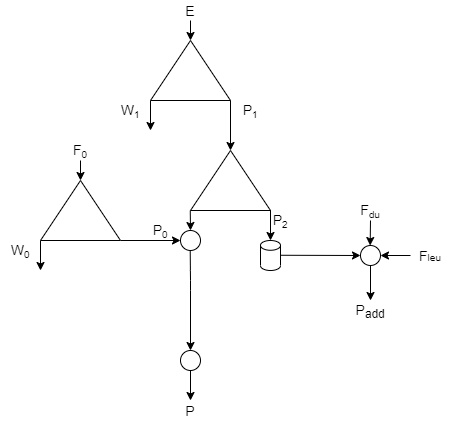
\includegraphics[scale=0.7]{cascades/P2utilization}}
  \caption{Схема независимого вовлечения загрязненногой изотопом $^{232}$U фракции с разбавлением обедненным и природным ураном}\label{P2utilization}
\end{figure}

Расчет целевых показателей схемы -- доли дополнительного НОУ-продукта, полученного из $P_2$, от новой ТВС (469 кг), а также экономии природного урана, производился на основе данных составов второго и пятого рециклов (см.постановку задачи), а также предположения двукратного увеличения предела содержания $^{232}$U в продукте, дополнительно произведенном из $P_2$ ($1\cdot10^{-7}$\% вместо $5\cdot10^{-7}$\%). Результаты вычислений представлены в таблице \ref{independent}.


\begin{table}[h]
  \centering
  \normalsize\begin{tabulary}{1.0\textwidth}{CCCCC}
  ПДК $^{232}$U & Цикл № & $P_2$, кг & Дополнительный продукт из $P_2$, доля новой ТВС, \% & Экономия природного урана, \% \\
  1.e-6\% & 2 & 1.09 & 7.11 & 14.6 \\
   & 5 & 0.92 & 10.21 & 6.3 \\
  5.e-7\% & 2 & 1.33 & 14.22 & 7.3 \\
   & 5 & 0.92 & 20.42 & 3.1 \\
  \end{tabulary}
  \caption{Результаты вовлечения $P_2$ в производство дополнительного НОУ-продукта. Обозначения: ПДК $^{232}$U -- предельно допустимая концентрация $^{232}$U в дополнительно производимом на основе $P_2$ продукте. {\label{independent}}}
\end{table}

Проведем анализ численных результатов расчета. Значения в столбце <<Дополнительный продукт из $P_2$, доля новой ТВС \%>> соответствуют доле дополнительно произведенного НОУ из побочного $P_2$, образовавшегося в процессе обогащения топлива из регенерата для одной ТВС (469 кг), а экономия природного урана приведена относительно схемы ординарного каскада для обогащения природного урана.

Как можно заключить из результатов, представленных в таблице \ref{independent}, предлагаемый способ использования $P_2$ через модификацию схемы двойного каскада с НОУ-разбавителем позволяет экономить дополнительное количество природного урана относительно двойного модифицированного каскада, в котором не предполагается задействование потока легкой фракции второго каскада. А эффект более значителен для случаев, когда задействуется побочный продукт $P_2$ двойного каскада, образующийся на начальных стадиях рециклирования уранового топлива. В рассматриваемом случае -- это второй рецикл (табл. \ref{independent}). Схема рис. \ref{P2utilization} также показывает себя как более предпочтительная в экономии природного урана (вдвое выигрышнее, согласно табл. \ref{independent}), когда предельно допустимая концентрация $^{232}$U в получаемом из $P_2$ конечном продукте допускается на уровне в два раза выше ($1\cdot10^{-7}$\% вместо $5\cdot10^{-7}$\%).  Значение экономии природного урана соответствует доле $P_2$, смешанной с обедненным ураном $F_{du}$, до того, как он будет смешан с НОУ-разбавителем $F_{leu}$, полученным из природного урана. Важно заметить, что значение этой доли соответствует экономии работы разделения, которая, в случае отказа от использования $P_2$, была бы затрачена на прямое обогащение природного урана в ординарном каскада для производства аналогичного замещающего количества свежего НОУ-продукта.

Итак, накопленный в ходе производства одной ТВС из регенерата побочный продукт $P_2$ можно использовать для производства дополнительных $\approx$7\% свежего НОУ-продукта от дополнительной топливной сборки. Это соответствует возможности произвести дополнительную 15-ю тепловыделяющую сборку из накопленного $P_2$, образовавшегося при производстве предыдущих четырнадцати ТВС. Таким образом, для современного легководного реактора, такого как, например, российский ВВЭР-1200 или европейский PWR, где активная зона состоит из более чем 150 тепловыделяющих сборок, взяв за основу предложенную схему, можно изготовить дополнительно более 10 ТВС. 



В качестве выводов, относящихся ко всем рассмотренным схемам, приведем следующие:
\begin{enumerate}
    \item схемы на основе двойного каскада, использующие НОУ-разбавитель, принципиально пригодны для решения задачи обогащения регенерированного урана в рамках многократного рецикла урановой составляющей топлива легководных реакторов. При этом каждая из схем имеет собственные достоинства и недостатки;
    \item характерным недостатком схемы, не предполагающей утилизацию нештатного отхода, образующегося в потоке $P_2$, является проблема с обращением с этим материалом, с высоким содержанием как четных изотопов (на 1-2 порядка выше, чем пределы для товарного НОУ) и $^{235}$U (до 20\% или, в некоторых случаях, до 90\%, в зависимости от выбранного режима работы каскадной схемы). Одним из вариантом обращения с ним, помимо схемы независимой утилизации побочного продукта легкой фракции второго каскада схемы двойного каскада с НОУ-разбавителем (рис. \ref{P2utilization}), может стать его перемешивание с отвалом первого каскада при обогащении регенерата. Оценки показали, что в этом случае возможно получить обедненный уран с приемлемым содержанием $^{232}$U (не выше $5\cdot10^{-7}$\%);
    \item характерными недостатком схемы двойного каскада с НОУ-разбавителем с возвратом потока $P_2$ в цикл (рис. \ref{P2utilizationRing}) является возврат значительной части четных изотопов на вход каскадной схемы;
    \item характерным недостатком схемы тройного каскада (рис. \ref{p2_withDepU}) являются дополнительные затраты работы разделения по отношению к схемам двойного каскада с НОУ-разбавителем, возникающие при обогащении разбавленного обедненным ураном отхода второго каскада схемы, загрязненного четными изотопами.
  \end{enumerate}

Анализ эффективности предложенных каскадных схем с точки зрения потерь $^{235}$U показал, что перспективными вариантами для дальнейшей технико-экономической проработки являются каскадные схемы двойного каскада с НОУ-разбавителем (рис. \ref{p2left}) и тройного каскада (рис. \ref{p2_withDepU}). Cхема двойного каскада с НОУ-разбавителем на каждом из рассмотренных рециклах позволяет извлечь более 80\% от массы $^{235}$U из исходного регенерированного урана, поступившего на обогащение.

Для каждой из предложенных схем разработаны оригинальные методики расчета и оптимизации ее переменных по критерию минимума расхода работы разделения каскадной схемы, основанная на использовании современных методов условной оптимизации функций многих переменных. С использованием разработанных методик расчета и оптимизации предложенных каскадных схем продемонстрирована возможность их использования для обогащения регенерированного урана в условиях многократного рецикла на примере взятого из литературы изотопного состава регенерата урана с повышенным содержанием четных изотопов и отвечающего пятому рециклу в топливе ВВЭР.

Для выбора конкретного варианта каскадной схемы для организации производственного процесса, необходим детальный технико-экономический анализ каждой из схем на основе их интегральных показателей, таких как расход сырьевых материалов и работы разделения, в контексте всей цепочки ядерного топливного цикла, а также с учетом возникающих в этой цепочке изменений при использовании регенерата урана по отношению к открытому топливному циклу. Помимо этого, необходима проработка технологических проблем каждой из схем, в частности, с точки зрения возможности эксплуатации и обслуживания оборудования в условиях работы с материалами, имеющими более высокую, чем природный уран удельную активность. Например, подобные условия возникают в каскадах, концентрирующие в легкой фракции $\alpha$-активные изотопы $^{232,234}$U. 



\clearpage